\documentclass[a4paper,11pt]{book}

% packages de base
\usepackage[french]{babel}
\usepackage[utf8]{inputenc}
\usepackage[T1]{fontenc}

% packages additionnels
\usepackage{array}  % Commandes complémentaires pour les tableaux
\usepackage{colortbl}  % Coloration des tableaux
\usepackage{fancyhdr}  % Personnalisation en-tête et pied de page
\usepackage[top=2.5cm, bottom=2.5cm, left=2.8cm, right=2.8cm]{geometry}  % Pour redimensionner les marges
\usepackage{graphicx}  % Pour les figures
\usepackage{multirow}  % Pour améliorer les tableaux
\usepackage{soul}  % Pour les soulignements
\usepackage{ulem}  % Pour les soulignements
\usepackage{color}  % Pour utiliser des couleurs
\usepackage{verbatim}  % Pour les citation de code
\usepackage{moreverb}  % Pour insérer du code avec tabulation
\usepackage{listings}  % Pour définir un environnement de citation de code
\usepackage{slashbox}  % Slashbox dans les cellules
\usepackage{url}  % Pour l'insertion des url
\usepackage{wrapfig}  % Pour intégrer des images dans un paragraphe

% les packs de polices
\usepackage{bookman}
\usepackage{charter}
\usepackage{newcent}
\usepackage{lmodern}
\usepackage{mathpazo}
\usepackage{mathptmx}

% Environnement pour du code Python:
\lstset{
    language=Python,
    basicstyle=\footnotesize,
    numbers=left,
    numberstyle=\normalsize,
    numbersep=4pt,
}
   
% Titre du livre
\title{\fbox{\LaTeX{} de A à X}}
\author{krystof}
\date{\today}

\begin{document}

\maketitle
\renewcommand{\contentsname}{Sommaire}
\tableofcontents

%%%%%%%%%%%%%%%%%%%%%%%%
%%% PREMIERE PARTIE  %%%
%%% Une présentation %%%
%%% de LaTeX.        %%%      
%%%%%%%%%%%%%%%%%%%%%%%%

\part{\textcolor{magenta}{Découvrir et installer \LaTeX}}

% Personnalisation en-têtes et pieds de pages
\pagestyle{fancy}
\renewcommand{\headrulewidth}{1pt}
\renewcommand{\headsep}{15pt}
\setlength{\headheight}{1cm}
\lhead{\textcolor{magenta}{Chapitre} \thechapter}
\rhead{\thepage}
\cfoot{}

%%%%%%%%%%%%%%%%%%%%%%%%%%%
%%% PART 1 - CHAPITRE 1 %%%
%%%%%%%%%%%%%%%%%%%%%%%%%%%

\chapter{Présentation de \LaTeX}
\section{\LaTeX, c'est...}
\LaTeX{} (se prononce \textit{latek}) est un langage créé originellement par des scientifiques qui cherchaient à rédiger des documents capables de gérer les mises en forme d'expression mathématiques, tout en offrant la possibilité d'y ajouter des extensions. Cette spécificité liée aux écritures mathématiques a rendu \LaTeX{} populaire parmi la communauté scientifique.

\begin{figure}[h]
\begin{center}
\includegraphics[scale=0.3]{IMG/LogoLaTex.jpeg}
\caption{Logo de \LaTeX}
\end{center}
\end{figure}

\LaTeX{} est un langage de balisage qu'il est aisé d'apprendre, et s'avère très utile. Au regard du rendu et de l'élégance des documents produits (mise en page de façon professionnelle), il offre de larges possibilités pour la rédaction d'articles, de mémoires, de thèses, mais aussi de livres. C'est en fait un langage de description qui permet de respecter les normes éditoriales et typographiques.
\medskip

Comparativement aux éditeurs de texte plus connus, tel que \textit{LibreOffice}, \LaTeX{} se montre bien plus efficace et aisé d'utilisation pour:
\begin{itemize}
\item la modification des styles de titres;
\item la gestion des notes;
\item la gestion des flottants (les figures que l'on insère dans les documents);
\item la rédaction et la gestion des longs documents;
\item la hiérarchisation du texte (parties, chapitres, sections, etc.);
\item la gestion des références internes au document;
\item la gestion des bibliographies, index et tables des matières.
\end{itemize}
\medskip

Avec \LaTeX{} tout est modifiable et paramétrable. De plus, nous pouvons à partir d'un document rédigé en \LaTeX de générer, par une simple compilation du fichier source \texttt{.tex}, des documents en \texttt{PDF}.
\medskip

\section{La petite histoire de \LaTeX}
Tout débute en 1977 par la création du langage \TeX{} par Donald Erwin \textsc{Knuth} qui cherchait alors à accroître la lisibilité et à optimiser l'insertion des formules mathématiques dans les articles scientifiques.
\medskip

En 1985, Leslie \textsc{Lamport} créé \LaTeX, bien plus aisé à utiliser que \TeX{}. Diverses tâches sont alors simplifiées à l'aide de macros intégrées au programme. Par la suite, suite à une évolution majeure, ce sera \LaTeXe{} qui sera majoritaire utilisé.
\medskip

%%%%%%%%%%%%%%%%%%%%%%%%%%%
%%% PART 1 - CHAPITRE 2 %%%
%%%%%%%%%%%%%%%%%%%%%%%%%%%

\chapter{Installer \LaTeX}
Une installation fonctionnelle comporte trois éléments:
\medskip

\begin{description}
\item[Une distribution \LaTeX]: le logiciel comprenant toutes les composantes nécessaires de \LaTeX.
\item[Un lecteur \texttt{PostScript} et/ou \texttt{PDF}]: afin de lire ses productions.
\item[Un éditeur \LaTeX]: qui facilite la rédaction d'un document rédigé en \LaTeX{}, même si un éditeur plus classique (exemple: \textit{Vim}) peut suffire.
\end{description}
\medskip

\section*{Installation sous \textit{Debian GNU/Linux}}
Pour la distribution \LaTeX{} on peut choisir d'installer le paquet \textit{texlive} (distribution de base) ou le paquet \textit{texlive-full} (distribution plus complète). On ajoutera le paquet \textit{cm-super} afin de disposer de polices supplémentaires.
\medskip

Pour lire et manipuler les fichiers \texttt{.ps} on installera \textit{gv}, et pour les fichiers \texttt{PDF} le lecteur \textit{evince} (bien intégré au bureau \textit{Gnome} sera suffisant.
\medskip

Enfin, concerant l'éditeur \LaTeX{} cela est souvent une question de goût et/ou d'habitude personnelle. Pour ma part ma préférence va au logiciel \textit{Texmaker}, qui dispose en plus d'une interface en français.
\medskip

%%%%%%%%%%%%%%%%%%%%%%%%%%%
%%% PART 1 - CHAPITRE 3 %%%
%%%%%%%%%%%%%%%%%%%%%%%%%%%

\chapter{Mécanisme et structuration d'un document \LaTeX}
\section{Un document à compiler}
Un document \LaTeX est avant tout du code qu'il est nécessaire de compiler pour obtenir un document lisible avec une mise en page élégante (du moins celle que l'on souhaite obtenir). Ce code se rédige dans un fichier \texttt{.tex} et la compilation, possible grâce à la distribution \LaTeX{} nous permettra de lire notre document au format \texttt{PS} ou \texttt{PDF}.
\medskip

Une compilation manuelle est tout à fait possible, mais pour un rendu quasi immédiat l'utilisation d'un éditeur \LaTeX{} facilite grandement notre travail.
\medskip

La rédaction d'un long document, tel un livre, nécessitera sûrement la création d'une bibliographie, d'un index, voire d'autres éléments complémentaires. Pour cela \LaTeX{} stocke de telles informations dans divers fichiers aux extensions différentes. La compilation de notre fichier \texttt{.tex} de départ générera alors une multitude de fichiers répondant aux besoins du document. 
\medskip

\section{Un premier document en guise d'exemple}
A l'aide d'un éditeur de texte \LaTeX{} saisir les lignes suivantes:
\begin{verbatim}
    \documentclass{article}
    
    \begin{document}
    Bonjour, voici donc un premier document très simple.
    \end{document}
\end{verbatim}
\medskip	

Il suffit ensuite d'enregistrer le fichier au format \texttt{.tex} dans un répertoire dédié. Le fichier doit ensuite être compilé, soit à l'aide de l'éditeur, ou bien sous GNU/Linux grâce à la ligne de commande. 
\medskip

Imaginons que nous ayons enregistré notre document sous le nom \texttt{document\_simple.tex}, voici comment le compiler et transformer les fichiers en celui voulu:
\begin{description}
	\item[\$ latex document\_simple.tex]: compilation qui permet d'obtenir le fichier \verb|document_simple.dvi|.
	\item[\$ xdvi document\_simple.dvi]: lecture du fichier grâce à la commande \verb|xdvi|.
	\item[\$ dvips document\_simple.dvi -o]: transformer le fichier \texttt{.dvi} en un fichier \texttt{.ps} grâce à la commande \verb|dvips|.
	\item[\$ ps2pdf document\_simple.ps]: transformation en un fichier \textit{PostScript}, grâce à la commande \verb|ps2pdf|.
	\item[\$ pdflatex document\_simple.tex]: compilation directe en un fichier \texttt{PDF} grâce à la commande \verb|pdflatex|.
	\item[\$ xpdf document\_simple.pdf]: lecture du fichier \texttt{PDF} grâce à la commande \verb|xpdf|.
\end{description}
\medskip

\section{Compilation et caractères spéciaux}
Comme tout langage de programmation, \LaTeX{} utilise certains caractères pour son usage propre. Il en existe dix. Insérer l'un de ces caractères dans votre texte et il en résultera des erreurs de compilation. La parade à cela est d'insérer un \textit{backslash} juste avant le caractère (Ex: \verb|\%|). Pour le \textit{backslash} lui-même nous utilisons la commande suivante: \verb|\textbackslash{}|.
\medskip

Les caractères spéciaux: \$ \& \% \# \_ \^{} \~{} \textbackslash{} \{ \}
\medskip

Il existe un nombre encore conséquent de caractères spéciaux utilisés dans un environnement mathématique et autres\footnote{\url{https://tice.univ-irem.fr/lexique/res/Annexe_E_-_Liste_des_symboles_mathematiques_usuels__LaTeX_.pdf}}.
\medskip

\section{Structuration d'un document \LaTeX}
Le texte de notre document doit impérativement s'insérer entre les deux lignes suivantes:
\begin{verbatim}
    \begin{document}
    \end{document}
\end{verbatim}
\medskip

\verb|\begin| et \verb|\end| délimitent ce que l'on nomme un environnement. Avec \LaTeX{} il existe divers environnements que nous découvrirons au fur et à mesure.
\medskip

\subsection*{Les divers types de documents}
La commande \verb|\documentclass{}| sert à indiquer à \LaTeX{} que le document que nous allons rédiger correspond à un certain type, et par conséquent \LaTeX{} va adapter sa mise en page au regard du type indiqué. Dans notre premier document simple donné en guise d'exemple, le type utilisé est \texttt{article}.
\medskip

Principaux types de document usités:
\begin{description}
	\item[article]: Article
	\item[book]: Livre
	\item[letter]: Lettre
	\item[report]: Rapport, thèse...
\end{description}
\medskip

Syntaxe de la commande \verb|documentclass{}| avec l'insertion d'options:
\begin{verbatim}
    \documentclass[options]{type}
\end{verbatim}
\medskip

%%%%%%%%%%%%%%%%%%%%%%%%%%%
%%% PART 1 - CHAPITRE 4 %%%
%%%%%%%%%%%%%%%%%%%%%%%%%%%

\chapter{Les packages}
\section{Que sont les packages ?}
Les packages sont des outils additionnels que l'on insère afin d'implémenter des fonctionnalités supplémentaires aux fonctionnalités de base. IL faut savoir que quand on utilise \LaTeX{} nous avons fréquemment recours aux packages. Ces packages sont disponibles sous deux formes: soit le package est déjà présent dans la distribution \LaTeX{} et il ne reste plus qu'à s'en servir, soit le package est absent et il sera alors nécessaire de l'installer. Il est à noter que les packages considérés comme incontournables sont installés par défaut dans la distribution \LaTeX{} de base.
\medskip

Pour utiliser un package on va se servir de la commande:
\begin{verbatim}
	\usepackage[option]{type}
\end{verbatim}  
\medskip

Cette commande se place juste après la commande \verb|\documentclass{}|.
\medskip

Exemple (noter l'utilisation du symbole \% pour insérer des commentaires):
\begin{verbatim}
	\documentclass{book}
	
	\usepackage[utf8]{inputenc}	  % un premier package
	\usepackage[T1]{fontenc}		     % un deuxième package
	\usepackage[french]{babel}	   % un troisième package
	
	\begin{document}
	    Mon texte...
	\end{document}
\end{verbatim}
\medskip

Dans notre exemple, les trois packages utilisés sont: \textit{babel}\footnote{Pour en apprendre un peu plus sur ce package, nous renvoyons à la partie consacrée aux packages de ce livre.} (Pour spécifier que le texte est écrit en français), \textit{fontenc} et \textit{inputenc} (pour utiliser tous les caractères du clavier). L'option \texttt{utf8} du package \textit{inputenc} s'accompagne, pour les linuxiens, de l'installation du paquet \textit{texlive-lang-french} de leur distribution GNU/Linux.
\medskip

\section{Installer un package non présent dans la distribution \LaTeX}
Ces packages sont portent souvent les extensions \texttt{.ins} et \texttt{.sty}. Certains packages peuvent porter une extension autre, et dans ce cas il faudra se reporter au fichier \texttt{README} qui les accompagne qui vous guidera dans l'installation.
\medskip

\subsection*{Au format \texttt{.sty}}
Pour l'installation d'un tel package, il suffit de copier le fichier dans le répertoire contenant le fichier \texttt{.tex} source. Lors de la compilation seront recherchés les fichiers \texttt{.sty}.
\medskip

\subsection*{Au format \texttt{.ins}}
L'installation se déroule en deux temps. Il faudra d'abord compiler le fichier \texttt{.ins}. Cette compilation va alors générer un fichier \texttt{.sty}. Placer ensuite ce fichier comme vu précédemment. 
\medskip


%%%%%%%%%%%%%%%%%%%%%%%%
%%% DEUXIEME PARTIE  %%%
%%% Pour une         %%%
%%% utilisation      %%%
%%% basique de LaTeX %%%      
%%%%%%%%%%%%%%%%%%%%%%%%

\part{\textcolor{magenta}{Pour une utilisation basique de \LaTeX}}

%%%%%%%%%%%%%%%%%%%%%%%%%%%
%%% PART 2 - CHAPITRE 5 %%%
%%%%%%%%%%%%%%%%%%%%%%%%%%%

\chapter{Commençons par la mise en page}
\section{La structure d'un document}
Nous allons ici apprendre à hiérarchiser notre document selon son type.
\medskip

\begin{table}[h]
\begin{center}
\begin{tabular}{|c|c|}
\hline
\textbf{Élément de structure} & \textbf{Code \LaTeX} \\
\hline
Partie & \verb|\part{Titre de la partie}| \\
\hline 
Chapitre & \verb|\chapter{Titre du chapitre}| \\
\hline
Section & \verb|\section{Titre de la section}| \\
\hline
Sous-section & \verb|\subsection{Titre de la sous-section}| \\
\hline
Paragraphe & \verb|\paragraph{Titre du paragraphe}| \\
\hline
Sous-paragraphe & \verb|\subparagraph{Titre du sous-paragraphe}| \\
\hline
\end{tabular}
\caption{Les différents niveaux de hiérarchisation}
\end{center}
\end{table}
\medskip

A noter que fonction du type de document certains niveaux de hiérarchisation ne sont pas accessibles (Exemple: Le niveau \textit{Chapitre} n'est par accessible pour le type \texttt{book}).
\medskip

Exemple\footnote{Le texte de notre exemple est extrait de la page \textit{Wikipedia} de \LaTeX .}:
\begin{verbatim}
    \documentclass{report}

    \usepackage[french]{babel}
    \usepackage[utf8]{inputenc}
    \usepackage[T1]{fontenc}
    
    \begin{document}
    \part{Première partie}
    \chapter{Premier chapitre}
    \section{Première section}
    \subsection{Première sous-section}
    \LaTeX{} permet de rédiger des documents dont la mise 	en page 
    est réalisée automatiquement en se conformant 	du mieux 
    possible à des normes typographiques. Une 		fonctionnalité 
    distinctive de \LaTeX{} est son mode 		mathématique, qui permet 
    de composer des formules complexes... 
    \end{document}
\end{verbatim}
\bigskip

\section{Les annexes}
Avec le type de document \texttt{book} ou \texttt{report}, nous avons fréquemment besoin d'ajouter des annexes. \LaTeX{} offre la possibilité d'une numérotation différente de celle des chapitres. Entre le contenu du texte (et à fortiori des divers chapitres) et les annexes, on va insérer la commande \verb|\appendix|.
\medskip

Exemple:
\begin{verbatim}
    \chapter{Premier}
    \chapter{Deuxième}
    \chapter{Troisième}
    \appendix % Les annexes débutent ici
    \chapter{Une première annexe}
    \chapter{Une seconde annexe}
\end{verbatim}
\medskip

Avec le type \texttt{article} la commande \verb|\appendix| influera sur le titre des sections.
\medskip

\section{Modifier la numérotation}
Il est possible de créer des chapitres sans numéro, ni lettre, en insérant une étoiles dans la commande: \verb|chapter*{Titre du chapitre}|. Cela fonctionne avec tous les éléments de structure.
\medskip

Nous pouvons aussi modifier le comportement de la numérotation à l'aide des commandes suivantes:
\begin{description}
\item[\textbackslash frontmatter]: Positionnée juste après la commande \verb|\begin{document}|, elle permet de numéroter le préambule en chiffres romains.
\item[\textbackslash mainmatter]: Entre le préambule et le premier chapitre, elle permet de lancer la numérotation habituelle des pages (en chiffres arabes).
\item[\textbackslash backmatter]: Positionnée avant le chapitre épilogue, les index et la bibliographie, elle stoppe la numérotation des chapitres, mais pas celle des pages.
\end{description}
\medskip

\section{Page de garde}
Elle se compose de trois éléments:
\begin{description}
\item[Le titre du document]: \verb|\title{Titre du document}|
\item[Le nom de l'auteur]: \verb|\author{Nom de l'auteur}|
\item[Une date]: \verb|\date{La date voulue}|
\end{description}
\medskip

Ces trois éléments sont insérés avec avant la commande \verb|\begin{document}|, et la commande \verb|\maketitle| placée juste après \verb|\begin{document}| permet de composer la page de garde. Il est bien sûr possible de réaliser des pages de garde bien plus complexes.
\medskip

\section{Les alignements de texte}
Avec \LaTeX{} les paragraphes sont naturellement justifiés. Ainsi pour tout autre type d'alignements les environnements suivants sont disponibles:
\begin{description}
\item[L'environnement \texttt{flushright}]: alignement du texte à droite.
\item[L'environnement \texttt{center}]: pour centrer le texte.
\item[L'environnement \texttt{flushleft}]: alignement du texte à gauche.
\end{description}
\medskip

\section{Les sauts de lignes}
Sauter deux lignes permet de créer un paragraphe:
\begin{verbatim}
    \begin{document}
    Un premier paragraphe
    
    Un second paragraphe
    \end{document}
\end{verbatim}
\medskip

Pour aller à la ligne sans crée de nouveau paragraphe on utilise la commande \verb|\newline| ou bien \verb|\\|. Pour faire un saut de page, c'est la commande \verb|\newpage|.
\medskip

\section{La commande \texttt{\textbackslash documentclass\{\}}}
\begin{table}[h]
\begin{center}
\begin{tabular}{|p{3.25cm}|p{4cm}|p{3.25cm}|}
\hline
\textbf{Description} & \textbf{Valeurs applicables} & \textbf{Valeur par défaut} \\
\hline
Format du papier & \texttt{a4paper}, \texttt{a5paper}, \texttt{letterpaper}, \texttt{b5paper}... & \texttt{letterpaper} \\
\hline
Taille de la police principale & \texttt{10pt}, \texttt{11pt}, \texttt{12pt} & \texttt{10pt} \\
\hline
Alignement des équations & \texttt{fleqn} (à gauche) & Centrées par défaut \\
\hline
Colonnes & \texttt{onecolumn}, \texttt{twocolumn} & \texttt{onecolumn} \\
\hline
Première page des chapitres & \texttt{openany}, \texttt{openright} & \texttt{openright} \\
\hline
Recto verso & \texttt{oneside}, \texttt{twoside} & \texttt{article} et \texttt{report}: \texttt{oneside} \& \texttt{book}: \texttt{twoside} \\
\hline
\end{tabular}
\caption{Options applicables à la commande \texttt{\textbackslash documentclass\{\}}}
\end{center}
\end{table}
\medskip

Il est tout à fait possible d'insérer plusieurs options à la fois, il suffit pour cela de les séparer par des virgules.
\medskip

\section{Les marges}
Pour modifier les marges nous allons tout d'abord utiliser la commande \verb|\layout| du package \textit{layout}. Saisir le code suivant et le compiler afin d'obtenir le \textit{layout} du document.
\begin{verbatim}
    \documentclass[a4paper,10pt]{book}

    \usepackage[french]{babel}
    \usepackage[utf8]{inputenc}
    \usepackage[T1]{fontenc}

    % packages additionnels
    \usepackage{layout}

    \begin{document}

    \layout

    \end{document}
\end{verbatim}
\medskip

\begin{table}[h]
\begin{center}
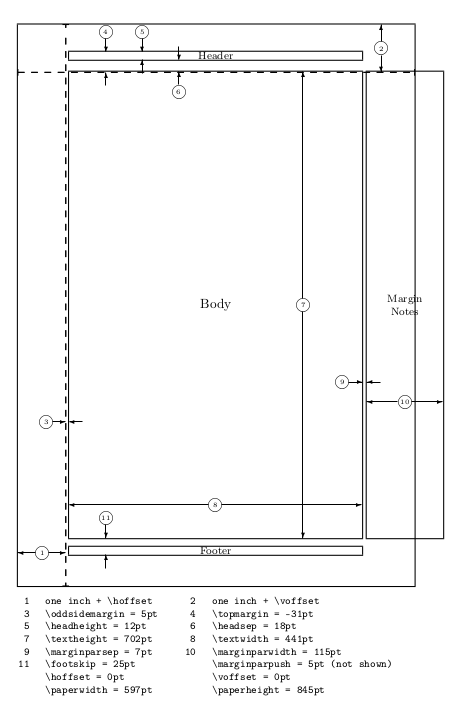
\includegraphics[scale=0.8]{IMG/layout.png}
\caption{Le \textit{layout}}
\end{center}
\end{table}
\medskip

Conjugué à un document saturé de texte nous pouvons visualiser le rendu avec les marges telles qu'elles sont définies. Nous pouvons alors modifier ces dernières à l'aide du package \textit{geometry}. Exemple de modification des marges à la fois en haut, en bas, à droite et à gauche, avec la ligne suivante placée dans la préambule du document:
\begin{verbatim}
    \usepackage[top=2.5cm, bottom=2.5cm, left=2.8cm, right=2.8cm]{geometry}
\end{verbatim}
\medskip

Il est toutefois possible d'intervenir encore plus finement en reprenant divers éléments du \textit{layout} qu'il est alors possible de modifier. Il suffit pour cela de placer dans le préambule une ligne du type:
\begin{verbatim}
    \setlength{nom_de_la_longueur}{longueur_dans_l'unité_voulue}
\end{verbatim}
\medskip

Un exemple:
\begin{verbatim}
    \setlength{\marginparwidth}{2cm}
\end{verbatim}
\medskip

\section{Les interlignes}
Les interlignes personnalisés s'obtiennent à l'aide du package \textit{setspace} et des commandes \verb|\onehalfspacing| et \verb|\doublespacing| qui permettent d'obtenir dans le document un interligne respectivement \textit{1,5} et \textit{2} fois plus grand que l'interligne habituel.
\medskip

Illustrons cela par le code suivant, à l'aide des environnement \texttt{onehalfspace} et \texttt{doublespace}:
\begin{verbatim}
    \documentclass[a4paper,11pt]{article}

    \usepackage[french]{babel}
    \usepackage[utf8]{inputenc}
    \usepackage[T1]{fontenc}

    \usepackage{setspace}

    \begin{document}
    \section{Interligne simple}
    \LaTeX{} est un langage et un système de composition de documents. 
    Il s'agit d'une collection de macro-commandes...
    
    \section{Interligne intermédiaire (\textit{1,5})}
    \begin{onehalfspace}
    \LaTeX{} est un langage et un système de composition de documents. Il 
    s'agit d'une collection de macro-commandes... 
    \end{onehalfspace}

    \section{Interligne double (\textit{2})}
    \begin{doublespace}
    \LaTeX{} est un langage et un système de composition de documents. Il 
    s'agit d'une collection de macro-commandes...
   \end{doublespace}
   \end{document}
\end{verbatim}
\medskip

\begin{table}[h]
\begin{center}
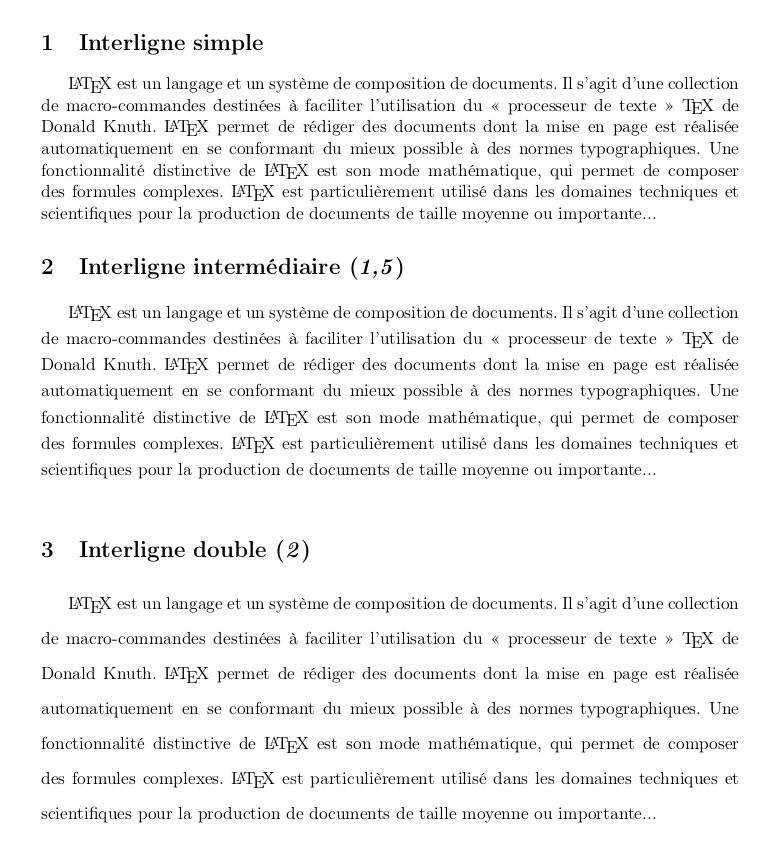
\includegraphics[scale=0.5]{IMG/interlignes.png}
\caption{Les interlignes}
\end{center}
\end{table}
\medskip

\section{Les listes}
Il existe les \textit{listes à puce}, les \textit{listes numérotées} et les \textit{les listes descriptives}. Chacune de ces listes s'insère dans un environnement spécifique. Plutôt que de partir sur de grandes explications, le principe étant aisé à comprendre, je vous propose de tester le code suivant:
\begin{verbatim}
    \documentclass[a4paper,11pt]{article}

    \usepackage[french]{babel}
    \usepackage[utf8]{inputenc}
    \usepackage[T1]{fontenc}

    \begin{document}
    \section{Les listes à puce}
    \begin{itemize}  % L'environnement des listes à puce
    \item Puce 1
    \item Puce 2
    \item Puce 3
    % Modifions les puces
    \item[@] Puce 4
    \item[5] Puce 5
    \item[*] Puce 6
    \item[\$] Puce 7
    \item[§] Puce 8
    \end{itemize}

    \section{Les listes numérotées}
    \begin{enumerate}  % L'environnement des listes numérotées
    \item Première
    \item Deuxième
    \item Troisième
    \end{enumerate}

    \section{Les listes descriptives}
    \begin{description}  % L'environnement des listes de description
    \item[Listes à puces]: avec l'environnement \textit{itemize}
    \item[Listes numérotées]: avec l'environnement \textit{enumerate}
    \item[Listes descriptives]: avec l'environnement \textit{description} 
    \end{description}
    \end{document}
\end{verbatim}
\medskip

\section{Les styles}
Pour peaufiner un peu plus nos mises en page nous allons voir maintenant les en-têtes et pieds de pages. De base, \LaTeX{} a été conçu avec trois modèles. Des packages proposent cependant des résultats plus aboutis, mais nous restons pour l'heure sur les modèles de base.
\medskip

Ces trois modèles sont donc:
\begin{description}
    \item[plain]: Ce style insère un numéro de page au milieu du pied de page.
    \item[headings]: Insère le nom du chapitre et le numéro de page en en-tête. Le pied de page demeure vide.
    \item[empty]: En-tête et pied de pages demeurent vides.
\end{description}
\medskip

Par défaut \LaTeX{} use du style \texttt{headings}. Pour modifier le style à une page en particulier, il suffit d'utiliser la commande \verb|\pagestyle{nom_du_style}| au début de la page.
\medskip

\section{Quelques règles}
Les commandes se terminant par des lettres doivent êtres suivies de la double accolade (\{\}) afin de pouvoir insérer une espace à leur suite (Exemple: \verb|\LaTeX{}|).
\medskip

%%%%%%%%%%%%%%%%%%%%%%%%%%%
%%% PART 2 - CHAPITRE 6 %%%
%%%%%%%%%%%%%%%%%%%%%%%%%%%

\chapter{Les polices}
Nous allons ici voir comment modifier la mise en forme d'un texte (en gars, en italique, surligné, etc...), changer la couleur d'un texte, et modifier aussi la police (ponctuellement ou définitivement).
\medskip

\section{La taille du texte}
\LaTeX{} propose dix commandes permettant d'augmenter ou de diminuer la taille d'un texte. On utilise ces commandes de deux manières:
\begin{verbatim}
    \commande{mon texte}
\end{verbatim}
\medskip

Ou:
\begin{verbatim}
    {\commande mon texte}
\end{verbatim}
\medskip

\begin{table}[h]
\begin{center}
\begin{tabular}{|c|c|}
\hline
\textbf{Commande} & \textbf{Taille du texte} \\
\hline
\verb|\tiny| & \tiny{Minuscule} \\
\hline
\verb|\scriptsize| & \scriptsize{Très très petit} \\
\hline
\verb|\footnotesize| & \footnotesize{Très petit} \\
\hline
\verb|\small| & \small{Petit} \\
\hline
\verb|\normalsize| & \normalsize{Normal} - Défini par défaut \\
\hline
\verb|\large| & \large{Un peu plus grand que normal} \\
\hline
\verb|\Large| & \Large{Grand} \\
\hline
\verb|\LARGE| & \LARGE{Très grand} \\
\hline
\verb|\huge| & \huge{Très très grand} \\
\hline
\verb|\Huge| & \Huge{Énorme !!!} \\
\hline
\end{tabular}
\caption{Les commandes pour les tailles de texte}
\end{center}
\end{table}
\medskip

\section{Graisse, italique, soulignement, etc.}
Nous disposons pour réaliser toutes ces opérations sur le texte de trois méthodes:
\begin{itemize}
    \item \verb|\commande{mon texte}|.
    \item \verb|{\comande mon texte}|.
    \item placer le texte dans un environnement.
\end{itemize}
\medskip

\begin{table}[h]
\begin{center}
\begin{tabular}{|c|c|c|}
\hline
\textbf{Mise en forme} & \textbf{Commandes} & \textbf{Rendu} \\
\hline
\multirow{2}*{Normal} & \verb|{\normalfont texte}| & {\normalfont texte} \\
& \verb|\begin{rm}texte\end{rm}| & \begin{rm}texte\end{rm} \\
\hline 
\multirow{3}*{Gras} & \verb|\textbf{texte}| & \textbf{texte} \\
& \verb|{\bfseries texte}| & {\bfseries texte} \\
& \verb|\begin{bf}texte\end{bf}| & \begin{bf}texte\end{bf} \\
\hline
\multirow{3}*{Italique} & \verb|\textit{texte}| & \textit{texte} \\
& \verb|{\itshape texte}| & {\itshape texte} \\
& \verb|\begin{it}texte\end{it}| & \begin{it}texte\end{it} \\
\hline
\multirow{3}*{Penché} & \verb|\textsl{texte}| & \textsl{texte} \\
& \verb|{\slshape texte}| & {\slshape texte} \\
& \verb|\begin{sl}texte\end{sl}| & \begin{sl}texte\end{sl} \\
\hline
\multirow{3}*{Machine à écrire} & \verb|\texttt{texte}| & \texttt{texte} \\
& \verb|{\ttfamily texte}| & {\ttfamily texte} \\
& \verb|\begin{tt}texte\end{tt}| & \begin{tt}texte\end{tt} \\
\hline
\multirow{4}*{Petites capitales} & \verb|\textsc{texte}| & \textsc{texte} \\
& \verb|\bsc{texte}| & \bsc{texte} \\
& \verb|{\scshape texte}| & {\scshape texte} \\
& \verb|\begin{sc}texte\end{sc}| & \begin{sc}texte\end{sc} \\
\hline
Exposant & \verb|texte\textsuperscript{texte}| & texte\textsuperscript{texte} \\
\hline
Encadré & \verb|\fbox{texte}| & \fbox{texte} \\
\hline
Soulignement & \multirow{2}*{\texttt{\textbackslash ul\{texte\}}} & \multirow{2}*{\ul{texte}} \\
\textit{package soul} & & \\
\hline
Soulignement & \multirow{2}*{\texttt{\textbackslash uuline\{texte\}}} & \multirow{2}*{\uuline{texte}} \\
\textit{package ulem} & & \\
\hline
Soulignement & \multirow{2}*{\texttt{\textbackslash uwave\{texte\}}} & \multirow{2}*{\uwave{texte}} \\
\textit{package ulem} & & \\
\hline
Barrer & \multirow{2}*{\texttt{\textbackslash st\{texte\}}} & \multirow{2}*{\st{texte}} \\
\textit{package soul} & & \\
\hline
\end{tabular}
\caption{Les diverses mises en forme du texte}
\end{center}
\end{table}
\medskip

\section{La commande \texttt{\textbackslash emph\{\}}}
Cette commande a un fonctionnement à part puisqu'elle permet d'indiquer à \LaTeX{} de mettre le texte en évidence (en emphase). C'est \LaTeX{} qui se chargera de choisir la meilleure manière de mettre le texte en valeur. Il est d'ailleurs préférable d'utiliser \verb|\emph{}| à l'italique.
\medskip

Nous pouvons cependant définir comment la commande \verb|\emph{}| va mettre en évidence la portion de texte voulue, en plaçant dans le préambule la ligne suivante:
\begin{verbatim}
    \renewcommand{\emph}{fonction_liée_à_la_commande}
\end{verbatim}
\medskip

Exemple pou une mise en évidence avec le style \og machine à écrire\fg{}: 
\begin{verbatim}
    \renewcommand{\emph}{\texttt}
\end{verbatim}
\medskip

\section{Mise en couleur}
\subsection*{Les couleurs par défaut}
Elles sont au nombre de huit et l'usage de la couleur nécessite l'emploi du package \textit{color}. Ces couleurs sont \texttt{black}, \texttt{white}, \texttt{red}, \texttt{green}, \texttt{blue}, \texttt{yellow}, \texttt{magenta} et \texttt{cyan}.
\medskip

La commande est la suivante:
\begin{verbatim}
    \textcolor{couleur}{mon texte}
\end{verbatim}
\medskip

\subsection*{Création de nouvelles couleurs}
Il est possible de créer de nouvelles couleurs avec la commande \verb|\definecolor| qui se place dans le préambule, soit à partir de niveaux de gris ou d'un mélange de trois couleurs (rouge, vert et bleu). Ces nouvelles couleurs se verront attribuer un nom et elles pourront s'utiliser grâce à la commande \verb|\textcolor|.
\medskip

\paragraph*{Par niveaux de gris}: Le niveau de gris se trouve sur une échelle située entre \texttt{0} (le noir) et le \texttt{1} (le blanc). Choisir un niveau de gris va consister à prendre un nombre à deux décimales situé entre \texttt{0} et \texttt{1}, que l'on va appliquer sur une des huit couleurs par défaut.
\begin{verbatim}
    \definecolor{nomchoisi}{une des 8 couleurs}{niveau de gris}
\end{verbatim}
\medskip

\paragraph*{Par mélange des trois couleurs}: Il suffit de choisir tour à tour l'intensité de rouge, de vert et de bleu (entre \texttt{0} et \texttt{1}).
\begin{verbatim}
    \definecolor{nomchoisi}{rgb}{taux de rouge, de ver, de bleu}
\end{verbatim}
\medskip

\section{Les packs de polices}
Afin de pouvoir changer les polices de caractères des packs de polices ont été créés, tout en ayant dans l'idée de conserver  une cohérence typographique à l'intégralité du texte. Un pack cohérent va comprendre quatre polices cohérentes:
\begin{itemize}
    \item des caractères avec empattements;
    \item des caractères sans empattements;
    \item des caractères façon machine à écrire;
    \item des caractères servant à écrire des formules mathématiques.
\end{itemize}
\medskip

Par défaut \LaTeX{} fournit la police \textit{Computer Modern}. Pour faire appel à autre pack c'est le même procédé que de faire appel à un package.
\begin{verbatim}
    \usepackage{nom_du_pack}
\end{verbatim}
\medskip

Des modifications ponctuelles de police peuvent aussi être introduites grâce à la commande:
\begin{verbatim}
    {\fontfamily{code_police}\selectfont mon texte}
\end{verbatim}
\medskip

Quelques packs: \textit{bookman}, \textit{charter}, \textit{newcent}, \textit{lmodern}, \textit{mathpazo}, \textit{mathptmx}, etc.
\begin{table}[h]
\begin{center}
\begin{tabular}{|c|c|}
\hline
\textbf{Code de la police} & \textbf{rendu} \\
\hline
\texttt{bch} & {\fontfamily{bch}\selectfont Mon texte en Charter} \\
\hline
\texttt{cmr} & {\fontfamily{cmr}\selectfont Mon texte en Computer Modern} \\
\hline
\texttt{lmr} & {\fontfamily{lmr}\selectfont Mon texte en Latin Modern Roman} \\
\hline
\texttt{lmss} & {\fontfamily{lmss}\selectfont Mon texte en Latin Modern Sans Empattement} \\
\hline
\texttt{lmmsq} & {\fontfamily{lmmsq}\selectfont Mon texte en Latin Modern Sans Emp. Exp.} \\
\hline
\texttt{lmtt} & {\fontfamily{lmtt}\selectfont Mon texte en Latin Modern Typewritter} \\
\hline
\texttt{pbk} & {\fontfamily{pbk}\selectfont Mon texte en Bookman} \\
\hline
\end{tabular}
\caption{Quelques exemples de polices}
\end{center}
\end{table}
\medskip

%%%%%%%%%%%%%%%%%%%%%%%%%%%
%%% PART 2 - CHAPITRE 7 %%%
%%%%%%%%%%%%%%%%%%%%%%%%%%%

\chapter{Citations, notes et références}
\section{Les citations}
Pour cela deux environnements sont proposés: \texttt{quote} et \texttt{quotation}.
\medskip

\texttt{quote} sera utilisé pour une citation simple:
\begin{verbatim}
    \begin{quote}
    La vie c'est comme une bicyclette, il faut avancer pour ne pas 
    perdre l'équilibre.
    \end{quote}
\end{verbatim}
\medskip

\begin{quote}
La vie c'est comme une bicyclette, il faut avancer pour ne pas perdre l'équilibre\footnote{Albert \textsc{Einstein}}.
\end{quote}
\medskip

\texttt{quotation} est fait pour de plus gros volumes de texte, et il introduit une tabulation comme pour un début de paragraphe.
\medskip
\begin{verbatim}
    \begin{quotation}
    Ainsi l'homme est si malheureux qu'il s'ennuierait même sans aucune cause 
    d'ennui par l'état propre de sa complexion. Et il est si vain qu'étant 
    plein de mille causes essentielles d'ennui, la moindre chose comme un 
    billard et une balle qu'il pousse suffisent pour le divertir.
    \end{quotation}
\end{verbatim}
\medskip

\begin{quotation}
Ainsi l'homme est si malheureux qu'il s'ennuierait même sans aucune cause d'ennui par l'état propre de sa complexion. Et il est si vain qu'étant plein de mille causes essentielles d'ennui, la moindre chose comme un billard et une balle qu'il pousse suffisent pour le divertir\footnote{Blaise \textsc{Pascal}}.
\end{quotation}
\medskip

\section{Les citations de code}
\subsection*{La commande \textbackslash \texttt{verb}}
Cette commande permet d'insérer du code dans un paragraphe:
\begin{verbatim}
    La commande \verb|\verb| pour insérer du texte.
\end{verbatim}
\medskip

Ce qui donne: La commande \verb|\verb| pour insérer du texte.
\medskip

Le caractère \texttt{|} peut être remplacé par \texttt{(} ou \texttt{[}:
\begin{verbatim} 
    \verb[mon code[
    \verb(mon code(
\end{verbatim}
\medskip

\subsection*{L'environnement \texttt{verbatim}}
Cet environnement s'accompagne du package \textit{verbatim}. Il permet d'accompagner de plus gros volumes de code, que l'on écrit généralement sur plusieurs lignes. Un point de vigilance à avoir: Les tabulations sont remplacées par des espaces.
\begin{verbatim}
\begin{verbatim}
# Une boucle Python
i = 0
while i < 5:
    print(i + " X 5 = " + (i*5))
    i =+ 1 
\end{verbatim}
\verb|\end{verbatim}|
\medskip

L'environnement \texttt{verbatimtab}, que l'on trouve avec le package \textit{moreverb}. La syntaxe est la suivante:
\begin{verbatim}
    \begin{verbatimtab}[nombre_d'espaces_par_tabulation]
    ...le code...
   \end{verbatimtab}
\end{verbatim}
\medskip

\subsection*{L'environnement \texttt{lstlisting}}
Cet environnement permet de mettre en forme du code avec de nombreuses et de façon colorée. Il est nécessaire d'utiliser le package \textit{listings} pour cela, puis de faire appel à la commande \texttt{lstset} dans l'en-tête du document. Cette sommande possède une grand nombre d'arguments paramétrables.
\begin{verbatim}
    \lstset{
    language=nom_du_langage,       % choix du langage
    basicstyle=\footnotesize,      % taille de la police du code
    numbers=left,                  % numéro des lignes placé à gauche
    numbers=right,                 % numéro des lignes placé à droite
    numberstyle=\normalsize,       % taille de la police des numéros
    numbersep=7pt,                 % distance entre code et numérotation
    backgroundcolor=\color{white}, % couleur de fond (utilisation du package 
                                   % 'color' possible)
    }
\end{verbatim}
\medskip

Les langages compatibles avec la commande sont constamment mis à jour sur la page \textit{Wikibooks} consacrée au package \textit{listings}\footnote{\url{https://en.wikibooks.org/wiki/LaTeX/Source_Code_Listings#Supported_languages}}.
\medskip

Le code à afficher s'insère dans l'environnement \texttt{lstlisting} comme ci-dessous avec un bout de code rédigé en langage \textit{Python}:
\begin{verbatim}
    \usepackage{listings}
    
    \lstset{
    language=Python,
    basicstyle=\footnotesize,
    numbers=left,
    numberstyle=\normalsize,
    numbersep=4pt,
    }
    
    \begin{document}
    
    \begin{lstlisting}
    # Une boucle while
    i = 0
    while i < 5:
        print(i + " X 5 = " + (i*5))
        i += 1
    \end{lstlisting}
    
    \end{document}
\end{verbatim}
\medskip

Ce qui donne à la compilation:
\begin{lstlisting}
    # Une boucle while
    i = 0
    while i < 5:
        print(i + " X 5 = " + (i*5))
        i += 1
\end{lstlisting}
\medskip

\section{Insérer une \textit{url}}
A l'aide du package \textit{url} et de la commande éponyme:
\begin{verbatim}
    \url{https://l'adresse_internet_à_faire_figurer}
\end{verbatim}
\medskip

\section{Texte encadré et l'environnement \texttt{minipage}}
L'environnement \texttt{minipage} et la commande \verb|\fbox| permettent d'encadrer du texte et de le mettre en valeur. Mais attention à les utiliser avec sobriété.
\medskip

\subsection*{Texte encadré avec \texttt{\textbackslash fbox}}
Avec \verb|\fbox| il est possible de paramétrer diverses choses. Nous allons ici en utiliser deux: l'écart entre le texte et la bordure et l'épaisseur de cette dernière.
\begin{verbatim}
    % Commande permettant de définir l'écart
    \setlength{\fboxsep}{8mm}
    % Commande permettant de définir l'épaisseur du trait
    \setlength{\fboxrule}{2mm}
    \fbox{Mon texte encadré}
\end{verbatim}
\medskip

Ce qui nous donne:
\begin{center}
\setlength{\fboxsep}{8mm}
\setlength{\fboxrule}{2mm}
\fbox{Mon texte encadré}
\end{center}
\medskip

\subsection*{L'environnement \texttt{minipage}}
Une \textit{minipage} est en encart de texte de largeur choisie, en quelque sorte une nouvelle page dans votre page. A l'intérieur de cet encart de texte, vous pourrez disposer et utiliser des environnements comme si cette \textit{minipage} était un document à part entière. L'environnement \texttt{minipage} est dépendant de deux paramètres: la largeur et l'alignement vertical.
\medskip

Illustrons cela:
\begin{verbatim}
  Voici mon texte dans lequel on insère une minipage
  \fbox{ % pour encadrer notre minipage
	  \begin{minipage}[c]{5cm}
	  au sein de laquelle je peux utiliser d'autres environnements:
		  \begin{center}
			  \LaTeX{} c'est \textbf{bien} !
		  \end{center}
	  \end{minipage}
  }
pour illustrer.
\end{verbatim}
\medskip

Voici mon texte dans lequel on insère une minipage
\fbox{
	\begin{minipage}[c]{5cm}
	au sein de laquelle je peux utiliser d'autres environnements:
		\begin{center}
			\LaTeX{} c'est \textbf{bien} !
		\end{center}
	\end{minipage}
}
pour illustrer.
\medskip

\section{Notes de bas de page}
\subsection*{La commande \texttt{\textbackslash footnote}}
A l'endroit où l'on souhaite insérer la note de bas de page:
\begin{verbatim}
    \footnote{Mon texte de bas de page}
\end{verbatim}
\medskip

\subsection*{La commande \textbackslash footnotemark}
Tout d'abord, marquer tous les éléments concernés par des notes de bas de page à l'aide d'un numéro, puis on insère le texte de bas de page correspondant au numéro. Deux compilations seront alors nécessaires.
\medskip

Exemple de code:
\begin{verbatim}
    Voici mon code\footnotemarck[1] qui permet d'insérer\footnotemark[2] 
    des notes de bas de page\footnotemark[3].
    
    % A insérer au niveau de la page où l'on souhaite voir figurer les 
    % notes de bas de page:
    \footnotetext[1]{Ma première note}
    \footnotetext[2]{Ma deuxième note}
    \footnotetext[3]{Ma troisième note}
\end{verbatim}
\medskip

\section{Les références internes}
\LaTeX{} permet d'écrire des références internes de façon simple à l'aide de trois commandes. La commande \verb|\label{nom_choisi}| sert à marquer un endroit, et les commandes \verb|\ref{nom_choisi}| et \verb|\pageref{nom_choisi}| permettent d'appeler le numéro de page ou la référence de l'élément marqué avec la commande \verb|\label{}|.
\medskip

%%%%%%%%%%%%%%%%%%%%%%%%%%%
%%% PART 2 - CHAPITRE 8 %%%
%%%%%%%%%%%%%%%%%%%%%%%%%%%

\chapter{Les figures}
\section{Choix des fichiers}
Avant d'entrer dans le vif du sujet voyons d'abord le type de compilation en fonction du fichier image utilisé.
\begin{description}
	\item[Utilisation de fichiers \texttt{.eps}]: obligation de compiler en \textit{Post-Script} avant d'effectuer une conversion en \textit{PDF}. Il sera impossible d'utiliser des fichiers \textit{PNG}, \textit{BMP}, \textit{jPEG} ou \textit{GIF} en parallèle.
	\item[Utilisation des fichiers \textit{PNG}, \textit{BMP}, \textit{jPEG} ou \textit{GIF}]: obligation de compiler directement en \textit{PDF}.
\end{description}
\medskip

Il est bien sût tout à fait possible de convertir un fichier image d'un format à une autre.
\medskip

\section{L'insertion d'image}
Tout d'abord il est nécessaire de faire appel au package \textit{graphicx}.
\medskip

La commande pour insérer simplement une figure:
\begin{verbatim}
    \includegraphics{chemin\du\fichier\image.xxx}
\end{verbatim}
\medskip

\section{Taille d'une image}
Il existe plusieurs méthodes pour indiquer à \LaTeX{} la taille de l'image à insérer:
\begin{itemize}
	\item faire en sorte que l'image ait une largeur donnée, la hauteur sera automatiquement adpatée;
	\item avec une hauteur donnée, c'est la largeur qui sera adaptée;
	\item fixer à la fois la hauteur et la largeur (risque de déformation de l'image);
	\item choisir un coefficient de proportionnalité et l'image sera \og retaillée\fg{} de façon cohérente.
\end{itemize}
\medskip

Les quatre commandes correspondantes:
\begin{verbatim}
    \includegraphics[width=200]{fichier_image.xxx}   % largeur
    \includegraphics[height=200]{fichier_image.xxx}  % hauteur
    \includegraphics[height=200, width=100]{fichier_image.xxx}  % fixation 
                     % hauteur et largeur
    \includegraphics[scale=1.5]{fichier_image.xxx}   % Avec coefficient
\end{verbatim}
\medskip

\section{Rotation d'une image}
On va pour cela utiliser la variable \texttt{angle}:
\begin{verbatim}
    \includegraphics[angle=45]{fichier_image.xxx}
\end{verbatim}
\medskip

\begin{figure}[h]
\begin{center}

\includegraphics[scale=0.25, angle=45]{IMG/tux.png}
\caption{Illustration avec un angle de 45°}
\end{center}
\end{figure}
\medskip

\section{Intégration d'une image dans un paragraphe}
Nous allons intégrer une image dans un texte de façon à ce que le texte contourne la figure à l'aide du package \textit{wrapfig} (afin d'utiliser l'environnement \texttt{wrapfigure}. Noter cependant que nous n'avons pas la pleine maîtrise du résultat car c'est \LaTeX{} qui redéfinit les arrangements. Avec l'environnement \texttt{wrapfigure} il existe diverses variables:
\begin{itemize}
	\item le nombre de lignes nécessaires à la bonne intégration de l'image;
	\item la taille du dépassement autorisé dans la marge (\texttt{0} pour garder des documents \og propres\fg{});
	\item la largeur de l'image;
	\item l'alignement de l'image. 
\end{itemize}
\medskip

La syntaxe est alors la suivante:
\begin{verbatim}
    \begin{wrapfigure}[nbre_de_lignes]{placement}{largeur_image_en_cm}
    \includegraphics[width=largeur_en_cm]{fichier_image.xxx}
    \end{wrapfigure}
    Mon paragraphe sans saut de ligne après la commande \end{wrapfigure}...
\end{verbatim}
\medskip

Le placement se définit à l'aide des lettres suivantes:
\begin{description}
    \item[l]: image à gauche;
    \item[r]: image à droite;
    \item[o]: image à l'extérieur (à droite avec une page impaire, à gauche avec une page paire);
    \item[i]: image à l'intérieur (à gauche pour une page impaire, à droite pour une page paire).
\end{description}
\medskip

Exemple de code pour intégrer une image de 2.5 x 2.3 cm de large, qui occupe 6 lignes et située à droite du paragraphe:
\begin{verbatim}
    \begin{wrapfigure}[6]{r}{2.5cm}
    
\includegraphics[width=2.3cm]{IMG/tux.png}
    \end{wrapfigure}
    Le paragraphe qui intègrera l'image...
\end{verbatim}
\medskip

Ce qui pourrait donner:
\medskip

\begin{wrapfigure}[6]{r}{2.5cm}

\includegraphics[width=2.3cm]{IMG/tux.png}
\end{wrapfigure}
La mascotte de \textit{Linux} est employée par de nombreuses applications en tant que logo, mais a aussi été modifiée par de nombreux particuliers et développeurs. On découvrira ainsi, parmi de nombreux autres, \textit{Tux} en Sherlock Holmes, en Dracula, ou encore en Charlie Chaplin ou habillé avec des maillots de football. De nombreux logiciels libres, comme \textit{TuxGuitar}, \textit{Tux Paint} ou \textit{Tux Racer} reprennent \textit{Tux} dans leur intitulé et/ou dans leur logo. Le dessin du personnage a été choisi à l'issue d'un concours organisé en 1996 remporté par Larry \textsc{Ewing}. Il utilisa \textit{GIMP}, le logiciel de traitement d'image phare sur \textit{GNU/Linux}. Il s'agit d'un personnage fictif représentant très approximativement un manchot pygmée dont l'idée a été suggérée par Alan \textsc{Cox1} puis affinée par Linus \textsc{Torvalds}, le créateur du noyau \textit{Linux}. Certains déclarèrent de prime abord que cette mascotte était inappropriée car elle n'évoquait guère la puissance. Linus \textsc{Torvalds} répondit que nulle personne poursuivie par un manchot pygmée, qui court vite et dispose d'un bec très dur, ne penserait cela. Les contradictions s'éteignirent...\footnote{Extrait de la page \textit{Wikipedia} consacrée à \textit{Tux}: \url{https://fr.wikipedia.org/wiki/Tux}.}
\medskip

%%%%%%%%%%%%%%%%%%%%%%%%%%%
%%% PART 2 - CHAPITRE 9 %%%
%%%%%%%%%%%%%%%%%%%%%%%%%%%

\chapter{Les flottants}
\LaTeX{} propose une façon optimisée pour placer des images et des figures, en spécifiant exactement leur place. C'est d'ailleurs une des fonctions phares de \LaTeX{}. Nous allons pour cela utiliser des environnements dits \og flottants\fg{}. En plus du positionnement ces environnements offrent la possibilité d'insérer des légendes à ces figures.
\medskip

Voyons donc cela avec l'environnement \texttt{figure}.
\medskip

\section{La création d'un flottant}
Très simplement, à l'aide de la commande \verb|\includegraphics{}| et l'environnement \texttt{figure}:
\begin{verbatim}
    \begin{figure}
    \begin{center}  % Pour centrer l'image
    \includegraphics{fichier_image.xxx}
    \end{center}    
    \end{figure} 
\end{verbatim}
\medskip

\section{Le placement}
Il est possible de spécifier le type de placement à l'aide d'options insérées dans l'environnement \texttt{figure}:
\begin{verbatim}
    \begin{figure}[option]
\end{verbatim}
\medskip

Les options de placement:
\begin{description}
	\item[t]: en haut de page;
	\item[b]: en bas de page;
	\item[p]: sur une page ne comportant que des flottants;
	\item[h]: placer de préférence dans la zone où l'on insère l'environnement;
	\item[H]: placer de façon insistante dans la zone où l'on insère l'environnement;
	\item[!b]: le \og !\fg{} pour insister encore plus;
	\item[bt]: de préférence en bas, mais en haut si en bas ce n'est pas possible. 
\end{description}
\medskip

\section{Le placement par défaut}
\LaTeX{} place les flottants par défaut suivant les options prévues, mais il est possible de modifier ce comportement à l'aide la de commande suivante, fournie par le package \texttt{float}:
\begin{verbatim}
    % Exemple avec un flottant de type 'figure'
    \floatplacement{figure}{t}
\end{verbatim}
\medskip

\section{Les légendes}
Pour légender des flottants on utilise la commande \verb|\caption{}|. Elle s'utilise à la suite de l'environnement \texttt{center} et précède une éventuelle commande \verb|\label{}|.
\begin{verbatim}
    \begin{figure}
    \begin{center}
    \includegraphics{fichier_image.xxx}
    \end{center}
    \caption{Texte de la légende}
    \label{référence}
    \end{figure}
\end{verbatim}
\medskip

\section{Les sauts de page avec le flottants}
\begin{description}
	\item[\texttt{\textbackslash clearpage}]: saut de page en produisant une page  remplie par tous les flottants non traités;
	\item[\texttt{\textbackslash cleardoublepage}]: même effet, si ce n'est que la nouvelle page sera nécessairement une page impaire.
\end{description}
\medskip

%%%%%%%%%%%%%%%%%%%%%%%%%%%%
%%% PART 2 - CHAPITRE 10 %%%
%%%%%%%%%%%%%%%%%%%%%%%%%%%%

\chapter{Les tableaux}
Il faut savoir que \LaTeX{} considère les tableaux comme des objets flottants. Les tableaux font l'objet d'une documentation extrêmement fournie, à l'instar de la documentation des notations mathématiques. Dans ce chapitre nous allons juste nous contenter d'apprendre à:
\begin{itemize}
	\item composer des tableaux simples;
	\item fusionner des cellules;
	\item paramétrer le placement allié à quelques détails de mise en page.
\end{itemize} 
\medskip

\section{Structure type d'un tableau}
\subsection*{Tableau sans bordure}
Nous allons utiliser l'environnement \texttt{tabular}. Dans un premier temps il faut décider de l'alignement des cellules dans chaque colonne (options):
\begin{description}
	\item[r]: à droite;
	\item[l]: à gauche;
	\item[c]: centré.
\end{description}
\medskip

Exemple de squelette de tableau à deux colonnes:
\begin{verbatim}
    \begin{tabular}{cc}
        ...code pour mon tableau...
    \end{tabular}
\end{verbatim}
\medskip

Nous entrons ensuite ligne par ligne le contenu des cellules, séparées par le caractère \texttt{\&}. Chaque ligne se termine par \textbackslash \textbackslash{} pour indiquer que nous changeons de ligne.
\medskip

Exemple de tableau à deux colonnes et deux lignes:
\begin{verbatim}
    \begin{tabular}{cc}
        lig. 1 col. 1 & lig. 1 col. 2 \\
        lig. 2 col. 1 & lig. 2 col. 2 \\
    \end{tabular}
\end{verbatim}
\medskip

Ce qui donne:
\begin{figure}[!h]
\begin{center}
\begin{tabular}{cc}
        lig. 1 col. 1 & lig. 1 col. 2 \\
        lig. 2 col. 1 & lig. 2 col. 2 \\
\end{tabular}
\end{center}
\end{figure}
\medskip

\subsection*{Tableau avec bordures}
Pour obtenir une ligne horizontale on va utiliser la commande \verb|\hline|. Pour marquer les colonnes, on va utiliser \og \texttt{|}\fg{} lors de la spécification des alignements.
\medskip

Exemple d'une tableau à deux colonnes et deux lignes:
\begin{verbatim}
    \begin{tabular}{|c|c|}
        \hline
        lig. 1 col. 1 & lig. 1 col. 2 \\
        \hline
        lig. 2 col. 1 & lig. 2 col. 2 \\
        \hline
    \end{tabular}
\end{verbatim}
\medskip

Ce qui donne:
\begin{figure}[!h]
\begin{center}
\begin{tabular}{|c|c|}
\hline
lig. 1 col. 1 & lig. 1 col. 2 \\
\hline
lig. 2 col. 1 & lig. 2 col. 2 \\
\hline
\end{tabular}
\end{center}
\end{figure}
\medskip

\section{Fusion des cellules}
\subsection*{Fusion de colonnes}
La commande est la suivante:
\begin{verbatim}
    \multicolumn{nbre_colonnes_fusionnées}{alignements}{Texte}
\end{verbatim}
\medskip

La difficulté réside dans le choix un nouvel alignement pour la cellule fusionnée.
\medskip

Illustrons cela:
\begin{verbatim}
    \begin{tabular}{|c|c|c|c|c|c|c|c|c|c|c|}
    \hline
    Multiplié par & 1 & 2 & 3 & 4 & 5 & 6 & 7 & 8 & 9 & 10 \\
    \hline
    1 & 1 & 2 & 3 & 4 & 5 & 6 & 7 & 8 & 9 & 10 \\
    \hline
    2 & 2 & 4 & 6 & 8 & 10 & 12 & 14 & 16 & 18 & 20 \\
    \hline
    3 & 3 & 6 & 9 & 12 & 15 & 18 & 21 & 24 & 27 & 30 \\
    \hline
    4 & 4 & 8 & 12 & 16 & 20 & 24 & 28 & 32 & 36 & 40 \\
    \hline
    5 & 5 & 10 & 15 & 20 & 25 & 30 & 35 & 40 & 45 & 50 \\
    \hline
    6 & 6 & 12 & 18 & 24 & 30 & 36 & 42 & 48 & 54 & 60 \\
    \hline
    7 & 7 & 14 & 21 & 28 & 35 & 42 & 49 & 56 & 63 & 70 \\
    \hline
    8 & 8 & 16 & 24 & 32 & 40 & 48 & 56 & 64 & 72 & 80 \\
    \hline
    9 & 9 & 18 & 27 & 36 & 45 & 54 & 63 & 72 & 81 & 90 \\
    \hline
    10 & 10 & 20 & 30 & 40 & 50 & 60 & 70 & 80 & 90 & 100 \\
    \hline 
\end{tabular}
\end{verbatim}
\begin{table}[!h]
\begin{center}
\begin{tabular}{|c|c|c|c|c|c|c|c|c|c|c|}
\hline
Multiplié par & 1 & 2 & 3 & 4 & 5 & 6 & 7 & 8 & 9 & 10 \\
\hline
1 & 1 & 2 & 3 & 4 & 5 & 6 & 7 & 8 & 9 & 10 \\
\hline
2 & 2 & 4 & 6 & 8 & 10 & 12 & 14 & 16 & 18 & 20 \\
\hline
3 & 3 & 6 & 9 & 12 & 15 & 18 & 21 & 24 & 27 & 30 \\
\hline
4 & 4 & 8 & 12 & 16 & 20 & 24 & 28 & 32 & 36 & 40 \\
\hline
5 & 5 & 10 & 15 & 20 & 25 & 30 & 35 & 40 & 45 & 50 \\
\hline
6 & 6 & 12 & 18 & 24 & 30 & 36 & 42 & 48 & 54 & 60 \\
\hline
7 & 7 & 14 & 21 & 28 & 35 & 42 & 49 & 56 & 63 & 70 \\
\hline
8 & 8 & 16 & 24 & 32 & 40 & 48 & 56 & 64 & 72 & 80 \\
\hline
9 & 9 & 18 & 27 & 36 & 45 & 54 & 63 & 72 & 81 & 90 \\
\hline
10 & 10 & 20 & 30 & 40 & 50 & 60 & 70 & 80 & 90 & 100 \\
\hline
\end{tabular}
\caption{Table de multiplication}
\end{center}
\end{table}
\medskip

\subsection*{Fusion de lignes}
Pour la fusion de lignes c'est la commande \verb|\multirow| contenue dans le package du même nom.
\begin{verbatim}
    \multirow{nbre de lignes fusionnées}{taille colonne en cm}{texte}
    \multirow{nbre de lignes fusionnées}*{texte}
\end{verbatim}

Observez bien le code suivant et le résultat qui s'en suit:
\begin{verbatim}
    \begin{tabular}{|l|c|c|c|c|}
    \hline
    1 & \multicolumn{2}{c|}{2} & 3 & 4 \\
    \hline
    \multicolumn{2}{|l|}{5} & 6 & 7 & 8 \\
    \hline
    9 & 10 & \multicolumn{3}{c|}{11} \\
    \hline
    \multirow{2}{1cm}{12} & 13 & 14 & 15 & 16 \\
    \cline{2-5}
    & 17 & 18 & 19 & 20 \\
    \hline
    21 & 22 & \multirow{2}*{23} & 24 & 25 \\
    \cline{1-2} \cline{4-5}
    26 & 27 & & 28 & 29 \\
    \hline
    \end{tabular}
\end{verbatim}
\medskip

\begin{table}[!h]
\begin{center}
\begin{tabular}{|l|c|c|c|c|}
\hline
1 & \multicolumn{2}{c|}{2} & 3 & 4 \\
\hline
\multicolumn{2}{|l|}{5} & 6 & 7 & 8 \\
\hline
9 & 10 & \multicolumn{3}{c|}{11} \\
\hline
\multirow{2}{1cm}{12} & 13 & 14 & 15 & 16 \\
\cline{2-5}
& 17 & 18 & 19 & 20 \\
\hline
21 & 22 & \multirow{2}*{23} & 24 & 25 \\
\cline{1-2} \cline{4-5}
26 & 27 & & 28 & 29 \\
\hline
\end{tabular}
\caption{Fusion de lignes et de colonnes}
\end{center}
\end{table}
\medskip

\section{Autres paramètres applicables à un tableau}
\subsection*{Colonne de largeur paramétrée}
\begin{verbatim}
    p{largeur de la colonne en centimètres}
\end{verbatim}
\medskip

Cette option n'a aucune influence sur l'alignement du texte au sein des cellules.
\medskip

Un exemple:
\begin{verbatim}
    \begin{tabular}{|p{1cm}|p{2cm}|p{3cm}|p{4cm}|}
    \hline
    1cm & 2cm & 3cm & 4cm \\
    \hline
    \end{tabular}
\end{verbatim}
\medskip

Ce qui donne:
\begin{table}[!h]
\begin{center}
\begin{tabular}{|p{1cm}|p{2cm}|p{3cm}|p{4cm}|}
    \hline
    1cm & 2cm & 3cm & 4cm \\
    \hline
\end{tabular}
\caption{Cellules de longueur définie}
\end{center}
\end{table}
\medskip

\subsection*{Créer une \textit{slashbox}}
Le package \textit{slashbox} permet d'utiliser la commande:
\begin{verbatim}
    \backslashbox{Texte dessous}{Texte dessus}
\end{verbatim}
\medskip

Cette commande sert à scinder en deux parties triangulaires de même aire une cellule initialement rectangulaire.
\medskip

Démonstration:
\begin{verbatim}
    \begin{tabular}{|c|p{1cm}|p{2cm}|}
    \hline
    \backslashbox{Debian}{Ubuntu} & 1cm & 2cm \\
    \hline
    \end{tabular}
\end{verbatim}
\medskip

Résultat:
\begin{table}
\begin{center}
\begin{tabular}{|c|p{1cm}|p{2cm}|}
\hline
\backslashbox{Debian}{Ubuntu} & 1cm & 2cm \\
\hline
\end{tabular}
\caption{Avec le package \textit{slashbox}}
\end{center}
\end{table}
\medskip

\subsection*{Changer les séparateurs}
Cela est possible à l'aide des commandes \verb|!{séparateur}| ou \verb|@{séparateur}|, contenues dans le package \textit{array}. A noter que ce package contient beaucoup de commandes utiles à la création des tableaux. La différence entre ces deux commandes réside dans le fait de pouvoir insérer une espace avant et après le séparateur.
\begin{verbatim}
    \begin{tabular}{|c !{\#} c @{\#}c|}
    \hline
    3 + 1 & = & 4 \\
    \hline
    \end{tabular}
\end{verbatim}
\medskip

Ce qui a pour résultat:
\begin{table}[!h]
\begin{center}
\begin{tabular}{|c !{\#} c @{\#}c|}
\hline
3 + 1 & = & 4 \\
\hline
\end{tabular}
\caption{De nouveaux séparateurs}
\end{center}
\end{table}
\medskip

\section{Des commandes et des environnements dans un tableau}
Démonstration avec la table de multiplication:
\begin{verbatim}
    \begin{tabular}{|>{\begin{bf}} c <{\end{bf}}|c|c|c|c|c|c|c|c|c|c|}
 
    \hline
    Multiplié par & \begin{bf}1\end{bf} & \begin{bf}2\end{bf} & 
    	\begin{bf}3\end{bf} & \begin{bf}4\end{bf} & \begin{bf}5\end{bf} & 
    	\begin{bf}6\end{bf} & \begin{bf}7\end{bf} & \begin{bf}8\end{bf} & 
    	\begin{bf}9\end{bf} & \begin{bf}10\end{bf} \\
    \hline
    1 & 1 & 2 & 3 & 4 & 5 & 6 & 7 & 8 & 9 & 10 \\
    \hline
    2 & 2 & 4 & 6 & 8 & 10 & 12 & 14 & 16 & 18 & 20 \\
    \hline
    3 & 3 & 6 & 9 & 12 & 15 & 18 & 21 & 24 & 27 & 30 \\
    \hline
    4 & 4 & 8 & 12 & 16 & 20 & 24 & 28 & 32 & 36 & 40 \\
    \hline
    5 & 5 & 10 & 15 & 20 & 25 & 30 & 35 & 40 & 45 & 50 \\
    \hline
    6 & 6 & 12 & 18 & 24 & 30 & 36 & 42 & 48 & 54 & 60 \\
    \hline
    7 & 7 & 14 & 21 & 28 & 35 & 42 & 49 & 56 & 63 & 70 \\
    \hline
    8 & 8 & 16 & 24 & 32 & 40 & 48 & 56 & 64 & 72 & 80 \\
    \hline
    9 & 9 & 18 & 27 & 36 & 45 & 54 & 63 & 72 & 81 & 90 \\
    \hline
    10 & 10 & 20 & 30 & 40 & 50 & 60 & 70 & 80 & 90 & 100 \\
    \hline
 
    \end{tabular}
\end{verbatim}
\medskip

Affichage:
\begin{table}[!h]
\begin{center}
\begin{tabular}{|>{\begin{bf}} c <{\end{bf}}|c|c|c|c|c|c|c|c|c|c|}
 
\hline
Multiplié par & \begin{bf}1\end{bf} & \begin{bf}2\end{bf} & \begin{bf}3\end{bf} & \begin{bf}4\end{bf} & \begin{bf}5\end{bf} & \begin{bf}6\end{bf} & \begin{bf}7\end{bf} & \begin{bf}8\end{bf} & \begin{bf}9\end{bf} & \begin{bf}10\end{bf} \\
\hline
1 & 1 & 2 & 3 & 4 & 5 & 6 & 7 & 8 & 9 & 10 \\
\hline
2 & 2 & 4 & 6 & 8 & 10 & 12 & 14 & 16 & 18 & 20 \\
\hline
3 & 3 & 6 & 9 & 12 & 15 & 18 & 21 & 24 & 27 & 30 \\
\hline
4 & 4 & 8 & 12 & 16 & 20 & 24 & 28 & 32 & 36 & 40 \\
\hline
5 & 5 & 10 & 15 & 20 & 25 & 30 & 35 & 40 & 45 & 50 \\
\hline
6 & 6 & 12 & 18 & 24 & 30 & 36 & 42 & 48 & 54 & 60 \\
\hline
7 & 7 & 14 & 21 & 28 & 35 & 42 & 49 & 56 & 63 & 70 \\
\hline
8 & 8 & 16 & 24 & 32 & 40 & 48 & 56 & 64 & 72 & 80 \\
\hline
9 & 9 & 18 & 27 & 36 & 45 & 54 & 63 & 72 & 81 & 90 \\
\hline
10 & 10 & 20 & 30 & 40 & 50 & 60 & 70 & 80 & 90 & 100 \\
\hline
 
\end{tabular}
\caption{Mise en gras de certaines parties}
\end{center}
\end{table}
\medskip

\subsection*{Colorer des cellules}
Pour cela deux packages sont nécessaires: \textit{color} et \textit{colortbl}. Les commandes sont les suivantes:
\begin{verbatim}
    \columncolor{couleur}  % Pour colorer les colonnes
    \rowcolor{couleur}  % Pour colorer des lignes
    \cellcolor{couleur}  % Pour colorer les cellules
\end{verbatim}
\medskip

Exemple d'un tableau avec la première ligne et la première colonne sur fond jaune:
\begin{verbatim}
    \begin{tabular}{>{\begin{bf} \columncolor{yellow}} c <{\end{bf}}cccccccccc}
    \hline  
    \rowcolor{yellow}Multiplié par & \begin{bf}1\end{bf} & \begin{bf}2\end{bf} & 
        \begin{bf}3\end{bf} & \begin{bf}4\end{bf} & \begin{bf}5\end{bf} & 
        \begin{bf}6\end{bf} & \begin{bf}7\end{bf} & \begin{bf}8\end{bf} & 
        \begin{bf}9\end{bf} & \begin{bf}10\end{bf} \\
    \hline 
    1 & 1 & 2 & 3 & 4 & 5 & 6 & 7 & 8 & 9 & 10 \\
    \hline
    2 & 2 & 4 & 6 & 8 & 10 & 12 & 14 & 16 & 18 & 20 \\
    \hline
    3 & 3 & 6 & 9 & 12 & 15 & 18 & 21 & 24 & 27 & 30 \\
    \hline
    4 & 4 & 8 & 12 & 16 & 20 & 24 & 28 & 32 & 36 & 40 \\
    \hline
    5 & 5 & 10 & 15 & 20 & 25 & 30 & 35 & 40 & 45 & 50 \\
    \hline
    6 & 6 & 12 & 18 & 24 & 30 & 36 & 42 & 48 & 54 & 60 \\
    \hline
    7 & 7 & 14 & 21 & 28 & 35 & 42 & 49 & 56 & 63 & 70 \\
    \hline
    8 & 8 & 16 & 24 & 32 & 40 & 48 & 56 & 64 & 72 & 80 \\
    \hline
    9 & 9 & 18 & 27 & 36 & 45 & 54 & 63 & 72 & 81 & 90 \\
    \hline
    10 & 10 & 20 & 30 & 40 & 50 & 60 & 70 & 80 & 90 & 100 \\
    \hline
    \end{tabular}
\end{verbatim}
\medskip

Affichage:
\begin{table}[!h]
\begin{center}
\begin{tabular}{>{\begin{bf} \columncolor{yellow}} c <{\end{bf}}cccccccccc}
\hline  
\rowcolor{yellow}Multiplié par & \begin{bf}1\end{bf} & \begin{bf}2\end{bf} & \begin{bf}3\end{bf} & \begin{bf}4\end{bf} & \begin{bf}5\end{bf} & \begin{bf}6\end{bf} & \begin{bf}7\end{bf} & \begin{bf}8\end{bf} & \begin{bf}9\end{bf} & \begin{bf}10\end{bf} \\
\hline 
1 & 1 & 2 & 3 & 4 & 5 & 6 & 7 & 8 & 9 & 10 \\
\hline
2 & 2 & 4 & 6 & 8 & 10 & 12 & 14 & 16 & 18 & 20 \\
\hline
3 & 3 & 6 & 9 & 12 & 15 & 18 & 21 & 24 & 27 & 30 \\
\hline
4 & 4 & 8 & 12 & 16 & 20 & 24 & 28 & 32 & 36 & 40 \\
\hline
5 & 5 & 10 & 15 & 20 & 25 & 30 & 35 & 40 & 45 & 50 \\
\hline
6 & 6 & 12 & 18 & 24 & 30 & 36 & 42 & 48 & 54 & 60 \\
\hline
7 & 7 & 14 & 21 & 28 & 35 & 42 & 49 & 56 & 63 & 70 \\
\hline
8 & 8 & 16 & 24 & 32 & 40 & 48 & 56 & 64 & 72 & 80 \\
\hline
9 & 9 & 18 & 27 & 36 & 45 & 54 & 63 & 72 & 81 & 90 \\
\hline
10 & 10 & 20 & 30 & 40 & 50 & 60 & 70 & 80 & 90 & 100 \\
\hline
\end{tabular}
\caption{Tableau avec des couleurs}
\end{center}
\end{table}
\medskip

\subsection*{L'environnement flottant \texttt{table}}
Cela revient à insérer l'environnement \texttt{tabular} dans un environnement flottant. Celui-ci se nomme \texttt{table} et est similaire en tout point à l'environnement \texttt{figure}, avec l'utilisation de \texttt{caption}, \texttt{label}, \texttt{center}, etc.
\medskip

%%%%%%%%%%%%%%%%%%%%%%%%%%%%
%%% PART 2 - CHAPITRE 11 %%%
%%%%%%%%%%%%%%%%%%%%%%%%%%%%

\chapter{Sommaire et index}
\section{Table des matières}
\subsection*{Table des matières simple}
Il suffit de placer la commande \verb|\tableofcontents| là où vous souhaitez insérer la table des matières. La table est conçue telle que le prévoient les paramètres par défaut de \LaTeX{}. cela nécessite deux compilations: la première permet à \LaTeX{} de comprendre la structure du document et de lister les titres, et la seconde permet la mise en forme de la table avec les numéros de pages.
\medskip

\subsection*{Paramétrage d'une table des matières}
\paragraph*{Appeler la table \og sommaire\fg{}}
avec la commande suivante à insérer dans le corps du document, juste avant la commande \verb|\tableofcontents|:
\begin{verbatim}
    \renewcommand{\contentsname}{Sommaire}
\end{verbatim}
\medskip

\paragraph*{Raccourcir une ligne}
Lors de la création d'un élément de structure il est possible de définir deux titres: l'un pour le document, l'autre pour la table des matières. On code cela de la manière suivante:
\begin{verbatim}
    \section{titre table des matières}{titre dans le document}
\end{verbatim}
\medskip

\paragraph*{Quel niveau hiérarchique dans notre table des matières ?}
Il est possible de définir le niveau hiérarchique de la table des matières (inclusion des sous-sections ou non, des sections, etc.). La commande à placer en préambule est alors la suivante:
\begin{verbatim}
    \setcounter{tocdepth}{Choix du niveau (nombre)}
\end{verbatim}
\medskip

Concernant le niveau hiérarchique choisi, voir le tableau suivant:
\begin{table}{!h}
\begin{center}
\begin{tabular}{|c|c|}
\hline
\textbf{Niveau hiérarchique (inclus)} & \textbf{Valeur} \\
\hline
Partie & -1 \\
\hline
Chapitre & 0 \\
\hline
Section & 1 \\
\hline
Sous-section & 2 \\
\hline
Sous-sous-section & 3 \\
\hline
Paragraphe & 4 \\
\hline
Sous-paragraphe & 5 \\
\hline
\end{tabular}
\caption{Tableau des niveaux hiérarchiques de la table des matières}
\end{center}
\end{table}
\medskip

A noter qu'avec la classe \texttt{book}, par défaut, les titres des paragraphes ne sont pas inclus.
\medskip

\section{Tables de figures et tableaux}
Ces tables suivent à peu prés les mêmes mécanismes que ceux de la table des matières. On utilise respectivement les commandes \verb|\listoffigures| et \verb|\listoftables|. Apparaissent dans ces tables, soit un titre spécialement conçu pour la table, soit la légende contenue dans la commande \verb|\caption{}|. Voici les deux usages de la commande \verb|\caption{}|:
\begin{verbatim}
    \caption{légende de la figure ou de la table}
    \caption[légende courte]{légende de la figure ou de la table}
\end{verbatim}
\medskip

Là encore, deux compilations sont nécessaires.
\medskip

\section{Les index}
La création d'un index nécessite le package \textit{makeindex} et l'insertion de la commande \verb|\makeindex| dans le préambule, puis on insère la commande \verb|\printindex| à l'endroit où l'on décide de l'afficher. Les entrées d'index seront marqués à l'aide de la commande \verb|\index{argument}| collée au mot que l'on souhaite indexé. L'utilisation d'index nécessite trois compilations. Dans l'index les \textit{arguments} figureront dans l'ordre alphabétique.
\medskip

Nous venons de voir la méthode la plus simple pour la création d'index, mais créer de véritables index s'avère beaucoup plus complexe.
\medskip

Commande permettant de d'insérer un \textit{argument} d'index avec une référence croisée:
\begin{verbatim}
    \index{argument|see{référence croisée}}
\end{verbatim}
\medskip


%%%%%%%%%%%%%%%%%%%%%%%%%
%%% TROISIEME PARTIE  %%%
%%% Vers une          %%%
%%% connaissance plus %%%
%%% approfondie de    %%%
%%% LaTeX             %%%
%%%%%%%%%%%%%%%%%%%%%%%%%

\part{\textcolor{magenta}{Vers une connaissance plus approfondie de \LaTeX}}
\chapter{La mise en page}
\section{Des en-têtes et pieds de pages personnalisés}
Nous allons réaliser cela à l'aide de la commande \verb|\pagestyle{fancy}| fournie par le package \textit{fancyhdr}. Cette commande découpe chaque en-tête et pied de page en trois morceaux, de sorte que nous devons personnaliser six commandes différentes pour arriver à créer une mise en page cohérente des en-têtes et pieds de pages.
\medskip

\begin{table}[h]
\begin{center}
\begin{tabular}{|c|c|}
\hline
\textbf{La commande} & \textbf{Son résultat} \\
\hline
\verb|\lhead{..}| & Gère le coin gauche de l'en-tête \\
\hline
\verb|\chead{..}| & Gère le centre de l'en-tête \\
\hline
\verb|\rhead{..}| & Gère le coin droit de l'en-tête \\
\hline
\verb|\lfoot{..}| & Gère le coin gauche du pied de page \\
\hline
\verb|\cfoot{..}| & Gère le centre du pied de page \\
\hline
\verb|\rfoot{..}| & Gère le coin droit du pied de page \\
\hline
\verb|\leftmark| & Nom du chapitre \\
\hline
\verb|\rightmark| & Nom de la section \\
\hline
\verb|\thepage| & Numéro de page \\
\hline
\verb|\thechapter| & Numéro du chapitre \\
\hline
\verb|\thesection| & Numéro de la section courante \\
\hline
\verb|\renewcommand{\headrulelewidth}{épaisseur}| & Épaisseur de la ligne entre l'en-tête et le corps du texte \\
\hline
\verb|\renewcommand{\footrulelewidth}{épaisseur}| & Épaisseur de la ligne entre le pied de page et le corps du texte \\
\hline
\verb|\renewcommand{\headsep}{longueur}| & Espacement entre l'en-tête et le corps du document \\
\hline
\end{tabular}
\caption{Les commandes disponibles avec le package \textit{fancyhdr}}
\end{center}
\end{table}
\medskip

Voici, à titre d'exemple, le style utilisé pour ce document (les lignes suivantes sont placés juste après la première ligne avec la commande \verb|\part{}|):
\begin{verbatim}
    % Personnalisation en-têtes et pieds de pages
    \pagestyle{fancy}
    \renewcommand{\headrulewidth}{1pt}
    \renewcommand{\headsep}{15pt}
    \setlength{\headheight}{1cm}
    \lhead{\textcolor{magenta}{Chapitre} \thechapter}
    \rhead{\thepage}
    \cfoot{}
\end{verbatim}
\medskip

\section{Les unités de longueur}
Le plus simple étant de préciser tout cela à l'aide du tableau ci-dessous:
\begin{table}[!h]
\begin{center}
\begin{tabular}{|l|c|c|}
\hline
\textbf{Unité} & \textbf{Exprimée avec \LaTeX{}} & \textbf{Valeur en millimètres} \\
\hline
Point & \texttt{pt} & 0,35 mm \\
\hline
Millimètre & \texttt{mm} & 1,00 mm \\
\hline
Pica & \texttt{pc} & 4,21 mm \\
\hline
Cicéro & \texttt{cc} & 4,53 mm \\
\hline
Centimètre & \texttt{cm} & 10,00 mm \\
\hline
Inch & \texttt{in} & 25.4 mm \\
\hline
\end{tabular}
\caption{Les unités de longueur}
\end{center}
\end{table}
\medskip

A titre d'indication une feuille A4 mesure 210 millimètres de large et 297 de haut.
\medskip

\section{Les espaces}
Ceux-ci peuvent se définir (entre deux mots, entre deux parties de texte) à l'aides des commandes suivantes:
\begin{table}[!h]
\begin{center}
\begin{tabular}{|p{3.5cm}|p{8.5cm}|}
\hline
\textbf{Commande} & \textbf{Résultat} \\
\hline
\verb|\hspace{longueur}| & Insère un espace horizontal de la longueur choisie. \\
\hline
\verb|\hspace*{longueur}| & Idem, saut que l'espace n'est pas inséré s'il y a un retour à la ligne entre les deux mots concernés par l'espacement. \\
\hline
\verb|\vspace{hauteur}| & Insère un espace vertical de la longueur choisie. \\
\hline
\verb|\vspace*{hauteur}| & Ici, l'espace n'est pas inséré s'il y a un saut de page. \\
\hline
\end{tabular}
\caption{Les quatre principales commandes d'espacement}
\end{center}
\end{table}
\medskip

\chapter{Les gabarits}
Voyons ici quelques gabarits dont il est tout à fait possible de vous inspirer.
\medskip

\section{La classe \texttt{article}}
\begin{verbatim}
    \documentclass[a4paper,10pt]{article}
    \usepackage[utf8x]{inputenc}
    \usepackage[T1]{fontenc}
    \usepackage[french]{babel}
    \usepackage{lmodern} % Pour changer le pack de police
    \author{\textsc{Nom} Prénom}
    \date{\today}
    \title{Mon titre d’article}

    \begin{document}
    
    \maketitle
    
    \begin{abstract}
    Le résumé (abstract en anglais) de mon article.
    \end{abstract}

    % Le contenu
    Bla bla bla

    \end{document}
\end{verbatim}
\medskip

\section{La classe \texttt{report}}
\begin{verbatim}
    \documentclass[a4paper,10pt]{report}
    \usepackage[utf8x]{inputenc}
    \usepackage[T1]{fontenc}
    \usepackage[french]{babel}
    \usepackage{lmodern} % Pour changer le pack de police
    \usepackage{makeidx}
    \title{Le titre}
    \author{\textsc{Nom} Prénom}
    \date{} % Pour mettre la date du jour, tapez \today
    \makeindex
    
    \begin{document}
    
    \maketitle
    
    \newpage
    \tableofcontents
    \newpage

    % Le contenu
    Bla\index{bla} bla bla

    \listoffigures
    \listoftables
    \printindex
    
    \end{document}
\end{verbatim}
\medskip

\section{La classe \texttt{book}}
\begin{verbatim}
    \documentclass{book}
    \usepackage[utf8]{inputenc}
    \usepackage[T1]{fontenc}
    \usepackage[french]{babel}
    \usepackage{lmodern} % Pour changer le pack de police
    \usepackage{makeidx}
    \makeindex
    \title{Le titre}
    \author{\textsc{Nom} Prénom}
    \date{\today}
    
    \begin{document}
    
    \maketitle % Page de garde
    
    \frontmatter
    
    Pages introductives
    
    \mainmatter
    
    Contenu
    
    \appendix
    
    Chapitres annexes
    % Certains mettent la bibliographie après backmatter.
    \bibliographystyle{} % Le style est mis entre crochets.
    \bibliography{bibli} % Mon fichier de base de données s’appelle bibli.bib.

    \backmatter

    Epilogue

    \tableofcontents
    \listoffigures
    \listoftables
    \printindex

    \end{document}
\end{verbatim}
\medskip

\section{La classe \texttt{letter}}
\begin{verbatim}
    \documentclass{letter}

    \usepackage[utf8]{inputenc}
    \usepackage[T1]{fontenc}
    \usepackage[francais]{babel}
    \usepackage{lmodern}

    \signature{M. Laleloulilo (signature)}
    \address{Première ligne de l’adresse \\ Deuxième ligne \\ Troisième ligne}

    \begin{document}
    % Pas besoin d’insérer un champ de datation. Il est ajouté par défaut.
    \begin{letter}{Un destinataire\\Un autre \\ Son copain \& son lapin \\
    ligne d’adresse 1 \\ ligne d’adresse 2 \\ ligne d’adresse 3}
    \opening{Formule de politesse d’ouverture,}

    Le texte.

    \closing{Cordialement, (formule de politesse)}
    \ps{P.-S. : Votre petit ajout ! :-)}
    
    \end{letter}
 
    \end{document}
\end{verbatim}
\medskip

\chapter{Les bibliographies}
Tout bon texte d'étude rédigé doit nécessairement comporter une bibliographie. \LaTeX{} offre à ce sujet des possibilités étendues, qui ne sont pas toujours aisées à aborder, mais les maîtriser ne donnera que plus de valeur à vos publications.
\medskip

\section{Le principe - Approche théorique}
Réaliser une bibliographie consiste à mettre en forme une liste d'ouvrages ou de publications. Il existe pour cela divers modèles bibliographiques\footnote{Nous renvoyons le lecteur vers la page \textit{Wikipedia} consacrée au sujet (\url{https://fr.wikipedia.org/wiki/Bibliographie}) et notamment la partie listant les divers types de bibliographies}. Retenons l'idée qu'\og \textit{une bibliographie est une liste structurée de références de documents, généralement écrits}\fg{}\footnote{Source \textit{Wikipedia}}.
\medskip

Concernant la réalisation d'une bibliographie avec \LaTeX{} il faut savoir que ce dernier utiliser pour cela un programme externe du nom de \texttt{Bib\TeX{}}. Ce programme fournit une armada d'outils destinés à concevoir facilement sa liste (la base de données) contenant toutes les informations sur les ouvrages (auteur, date de parution, etc.). Chaque ouvrage se voit affecté une étiquette et il suffira d'intégrer cette étiquette dans le document \texttt{.tex} pour que l'ouvrage en question figure dans le document rédigé.
\medskip

Les étapes de ce principe:
\begin{enumerate}
	\item Création d'une base de données (listing des ouvrages et publications). Chaque ouvrage se voit affecté une étiquette.
	\item Les étiquettes sont insérées dans le texte.
	\item Les différents ouvrages appelés dans le manuscrit sont sélectionnés dans la base de données.
	\item La bibliographie est créée dans le document.
\end{enumerate}
\medskip

\section{La base de données}
Cette base de données est constituée de paragraphes contenant chacun les informations et l'étiquette des ouvrages. Le fichier qui sera enregistré le sera au format \texttt{.bib}. La structuration des informations concernant un ouvrage dans une base de données est toujours la même:
\begin{verbatim}
    @type_d'oeuvre{référence_courte,
    Titre_du_champ1={Texte},
    Titre_du_champ2={Texte},
    Titre_du_champ2={Texte},
    Titre_du_champ2={Texte},
    }
    Entre deux ouvrages, tout texte est considéré comme commentaire.
    @type_d'oeuvre{référence_courte,
    Titre_du_champ1={Texte},
    Titre_du_champ2={Texte},
    Titre_du_champ2={Texte},
    Titre_du_champ2={Texte},
    }
\end{verbatim}
\medskip

\begin{table}[!h]
\begin{center}
\begin{tabular}{|p{3.5cm}|p{3.5cm}|p{6cm}|}
\hline
\textbf{Type d'oeuvre} & \textbf{Correspondance} & \textbf{Champs disponibles} \\
\hline
\verb|@article| & Article & \texttt{author}, \texttt{journal}, \texttt{title}, \texttt{year}, \texttt{month}, \texttt{pages}, \texttt{notes} \\
\hline
\verb|@book| & Livre & \texttt{author}, \texttt{title}, \texttt{publisher}, \texttt{year} \\
\hline
\verb|@manual| & Document technique & \texttt{title}, \texttt{author}, \texttt{year}, \texttt{organization} \\
\hline
\verb|@misc| & Divers & \texttt{author}, \texttt{title}, \texttt{year}, \texttt{month}, \texttt{note} \\
\hline
\verb|@phdtheisis| & Thèse de doctorat & \texttt{author}, \texttt{title}, \texttt{school}, \texttt{year} \\
\hline
\verb|@unpublished| & Manuscrit non publié & \texttt{author}, \texttt{title}, \texttt{note}, \texttt{year}, \texttt{month} \\
\hline
\end{tabular}
\caption{Les types d'oeuvres et les champs disponibles, parmi les plus répandus.}
\end{center}
\end{table}
\medskip

Pour le champ \texttt{author}, les noms et les prénoms sont séparés par une virgule, et quand il y a plusieurs auteurs ils sont eux séparés par l'instruction \texttt{AND}.
\medskip

\begin{table}[!h]
\begin{center}
\begin{tabular}{|c|l|}
\hline
\textbf{Champs} & \textbf{Correspondance} \\
\hline
\texttt{author} & Auteur \\
\hline
\texttt{journal} & Journal \\
\hline
\texttt{month} & Mois de publication au choix (\textbf{jan}, \texttt{feb}, \texttt{mar}...) \\
\hline
\texttt{note} & Notes complémentaires \\
\hline
\texttt{organization} & Société ou organisation \\
\hline
\texttt{pages} & Pages concernées \\
\hline
\texttt{publisher} & Editeur \\
\hline
\texttt{year} & Année de publication \\
\hline
\end{tabular}
\caption{Les principaux champs.}
\end{center}
\end{table}
\medskip

Exemple pour article de revue:
\begin{verbatim}
    @article{ref,
    author={Durand, Patrick AND Durand, René},
    journal={La gazette linuxienne},
    title={La distribution qui va détrôner Windows...},
    year={2022},
    months={jun},
    pages={8},
    notes={Complément paramétrages}
    }
\end{verbatim}
\medskip

Exemple pour un livre:
\begin{verbatim}
    @book{ref,
    author={Kerouac, Jack},
    title={Sur la route},
    publisher={Gallimard},
    year={1976}
    }
\end{verbatim}
\medskip

\section{Mise en place de la bibliographie}
Nous ferons référence à des éléments de la base de données via la commande:
\begin{verbatim}
    \cite{référence courte} 
\end{verbatim} \\

que nous placerons à l'endroit désiré dans le texte. Cette commande est à allier avec les commandes:
\begin{verbatim}
    \bibliographystyle{style}
    \bibliography{nom fichier .bib (sans.bib)}
\end{verbatim}
\medskip

Exemple:
\begin{verbatim}
    \begin{document}
    
    Mon texte est issue de l'ouvrage \cite{ref} qui s'appuie lui même sur 
    le livre \cite{ref2}...

    \bibliographystyle{un des styles}
    \bibliography{ma_bibli}
    
    \end{document}        
\end{verbatim}
\medskip

\verb|\bibliographystyle{style}| utilise divers styles que nous pouvons résumer dans le tableau ci-dessous:
\begin{table}[!h]
\begin{center}
\begin{tabular}{|p{2cm}|p{10cm}|}
\hline
\textbf{Styles} & \textbf{Effets} \\
\hline
\texttt{plain}  & Classe les entrées par ordre alphabétique et les numérote en conséquence. \\
\hline
\texttt{abbrv} & Classe les entrées par ordre alphabétique, les numérote en conséquence et abrège certains éléments de la bibliographie. \\
\hline
\texttt{unsrt} & Trie les entrées par ordre d'apparition dans le texte. \\
\hline
\texttt{alpha} & Le repère n'est plus un chiffre, mais les trois premières lettres du nom de l'auteur accolées aux derniers chiffres de l'année de parution. \\
\hline
\end{tabular}
\caption{Les styles bibliographiques}
\end{center}
\end{table}
\medskip

\section{La compilation} 
La compilation d'une bibliographie va se dérouler en plusieurs temps. Deux compilations du fichier \texttt{.tex} source seront d'abord nécessaire, avant la compilation du fichier \texttt{.bib}, puis à nouveau deux autres compilations du fichier \texttt{.tex}.
\medskip

Sous \textit{GNU/Linux} cela donne:
\begin{verbatim}
    $ latex fichier_source.tex
    $ latex fichier_source.tex
    $ bibtex fichier.bib
    $ latex fichier_source.tex
    $ latex fichier_source.tex
\end{verbatim}
\medskip

\chapter{Structurer son document avec plusieurs fichiers \texttt{.tex}}
\section{Le concept}
Pour les longs documents (tel celui-ci) il est possible de les scinder en plusieurs fichiers \texttt{.tex}. Cela permet de travailler sur une partie sans toucher aux autres. Ce principe repose sur une simple commande:
\begin{verbatim}
    \input{chemin_du_fichier}
\end{verbatim}
\medskip

Avec cette commande, \LaTeX{} insère alors le contenu du fichier appelé.
\medskip

\section{Illustration par un exemple fictif}
Il faut tout d'abord créer la structure de fichiers du projet de notre document:
\begin{verbatim}
	Répertoire principal
	    |__ Fichier .tex principal
	    |
	    |__ Répertoire "Part1"
	    |        |__ Fichier "chapitre1.tex"
	    |        |__ Fichier "chapitre2.tex"
	    |
	    |__ Répertoire "Part2"
	             |__ Fichier "chapitre3.tex"
	             |__ Fichier "chapitre4.tex"
\end{verbatim}
\medskip

Le fichier \texttt{.tex} principal contiendra alors les lignes suivantes:
\begin{verbatim}
    \documentclass[book]
    
    % Insertion des lignes de préambule
    
    \begin{document}
    
    \part{Première partie}
    %%%%%%%%%%%%%%%%%%%%%%%%%%%
%%% PART 1 - CHAPITRE 1 %%%
%%%%%%%%%%%%%%%%%%%%%%%%%%%

\chapter{Présentation de \LaTeX}
\section{\LaTeX, c'est...}
\LaTeX{} (se prononce \textit{latek}) est un langage créé originellement par des scientifiques qui cherchaient à rédiger des documents capables de gérer les mises en forme d'expression mathématiques, tout en offrant la possibilité d'y ajouter des extensions. Cette spécificité liée aux écritures mathématiques a rendu \LaTeX{} populaire parmi la communauté scientifique.

\begin{figure}[h]
\begin{center}
\includegraphics[scale=0.3]{IMG/LogoLaTex.jpeg}
\caption{Logo de \LaTeX}
\end{center}
\end{figure}

\LaTeX{} est un langage de balisage qu'il est aisé d'apprendre, et s'avère très utile. Au regard du rendu et de l'élégance des documents produits (mise en page de façon professionnelle), il offre de larges possibilités pour la rédaction d'articles, de mémoires, de thèses, mais aussi de livres. C'est en fait un langage de description qui permet de respecter les normes éditoriales et typographiques.
\medskip

Comparativement aux éditeurs de texte plus connus, tel que \textit{LibreOffice}, \LaTeX{} se montre bien plus efficace et aisé d'utilisation pour:
\begin{itemize}
\item la modification des styles de titres;
\item la gestion des notes;
\item la gestion des flottants (les figures que l'on insère dans les documents);
\item la rédaction et la gestion des longs documents;
\item la hiérarchisation du texte (parties, chapitres, sections, etc.);
\item la gestion des références internes au document;
\item la gestion des bibliographies, index et tables des matières.
\end{itemize}
\medskip

Avec \LaTeX{} tout est modifiable et paramétrable. De plus, nous pouvons à partir d'un document rédigé en \LaTeX de générer, par une simple compilation du fichier source \texttt{.tex}, des documents en \texttt{PDF}.
\medskip

\section{La petite histoire de \LaTeX}
Tout débute en 1977 par la création du langage \TeX{} par Donald Erwin \textsc{Knuth} qui cherchait alors à accroître la lisibilité et à optimiser l'insertion des formules mathématiques dans les articles scientifiques.
\medskip

En 1985, Leslie \textsc{Lamport} créé \LaTeX, bien plus aisé à utiliser que \TeX{}. Diverses tâches sont alors simplifiées à l'aide de macros intégrées au programme. Par la suite, suite à une évolution majeure, ce sera \LaTeXe{} qui sera majoritaire utilisé.
\medskip

    %%%%%%%%%%%%%%%%%%%%%%%%%%%
%%% PART 1 - CHAPITRE 2 %%%
%%%%%%%%%%%%%%%%%%%%%%%%%%%

\chapter{Installer \LaTeX}
Une installation fonctionnelle comporte trois éléments:
\medskip

\begin{description}
\item[Une distribution \LaTeX]: le logiciel comprenant toutes les composantes nécessaires de \LaTeX.
\item[Un lecteur \texttt{PostScript} et/ou \texttt{PDF}]: afin de lire ses productions.
\item[Un éditeur \LaTeX]: qui facilite la rédaction d'un document rédigé en \LaTeX{}, même si un éditeur plus classique (exemple: \textit{Vim}) peut suffire.
\end{description}
\medskip

\section*{Installation sous \textit{Debian GNU/Linux}}
Pour la distribution \LaTeX{} on peut choisir d'installer le paquet \textit{texlive} (distribution de base) ou le paquet \textit{texlive-full} (distribution plus complète). On ajoutera le paquet \textit{cm-super} afin de disposer de polices supplémentaires.
\medskip

Pour lire et manipuler les fichiers \texttt{.ps} on installera \textit{gv}, et pour les fichiers \texttt{PDF} le lecteur \textit{evince} (bien intégré au bureau \textit{Gnome} sera suffisant.
\medskip

Enfin, concerant l'éditeur \LaTeX{} cela est souvent une question de goût et/ou d'habitude personnelle. Pour ma part ma préférence va au logiciel \textit{Texmaker}, qui dispose en plus d'une interface en français.
\medskip

    
    \part{Seconde partie}
    %%%%%%%%%%%%%%%%%%%%%%%%%%%
%%% PART 1 - CHAPITRE 3 %%%
%%%%%%%%%%%%%%%%%%%%%%%%%%%

\chapter{Mécanisme et structuration d'un document \LaTeX}
\section{Un document à compiler}
Un document \LaTeX est avant tout du code qu'il est nécessaire de compiler pour obtenir un document lisible avec une mise en page élégante (du moins celle que l'on souhaite obtenir). Ce code se rédige dans un fichier \texttt{.tex} et la compilation, possible grâce à la distribution \LaTeX{} nous permettra de lire notre document au format \texttt{PS} ou \texttt{PDF}.
\medskip

Une compilation manuelle est tout à fait possible, mais pour un rendu quasi immédiat l'utilisation d'un éditeur \LaTeX{} facilite grandement notre travail.
\medskip

La rédaction d'un long document, tel un livre, nécessitera sûrement la création d'une bibliographie, d'un index, voire d'autres éléments complémentaires. Pour cela \LaTeX{} stocke de telles informations dans divers fichiers aux extensions différentes. La compilation de notre fichier \texttt{.tex} de départ générera alors une multitude de fichiers répondant aux besoins du document. 
\medskip

\section{Un premier document en guise d'exemple}
A l'aide d'un éditeur de texte \LaTeX{} saisir les lignes suivantes:
\begin{verbatim}
    \documentclass{article}
    
    \begin{document}
    Bonjour, voici donc un premier document très simple.
    \end{document}
\end{verbatim}
\medskip	

Il suffit ensuite d'enregistrer le fichier au format \texttt{.tex} dans un répertoire dédié. Le fichier doit ensuite être compilé, soit à l'aide de l'éditeur, ou bien sous GNU/Linux grâce à la ligne de commande. 
\medskip

Imaginons que nous ayons enregistré notre document sous le nom \texttt{document\_simple.tex}, voici comment le compiler et transformer les fichiers en celui voulu:
\begin{description}
	\item[\$ latex document\_simple.tex]: compilation qui permet d'obtenir le fichier \verb|document_simple.dvi|.
	\item[\$ xdvi document\_simple.dvi]: lecture du fichier grâce à la commande \verb|xdvi|.
	\item[\$ dvips document\_simple.dvi -o]: transformer le fichier \texttt{.dvi} en un fichier \texttt{.ps} grâce à la commande \verb|dvips|.
	\item[\$ ps2pdf document\_simple.ps]: transformation en un fichier \textit{PostScript}, grâce à la commande \verb|ps2pdf|.
	\item[\$ pdflatex document\_simple.tex]: compilation directe en un fichier \texttt{PDF} grâce à la commande \verb|pdflatex|.
	\item[\$ xpdf document\_simple.pdf]: lecture du fichier \texttt{PDF} grâce à la commande \verb|xpdf|.
\end{description}
\medskip

\section{Compilation et caractères spéciaux}
Comme tout langage de programmation, \LaTeX{} utilise certains caractères pour son usage propre. Il en existe dix. Insérer l'un de ces caractères dans votre texte et il en résultera des erreurs de compilation. La parade à cela est d'insérer un \textit{backslash} juste avant le caractère (Ex: \verb|\%|). Pour le \textit{backslash} lui-même nous utilisons la commande suivante: \verb|\textbackslash{}|.
\medskip

Les caractères spéciaux: \$ \& \% \# \_ \^{} \~{} \textbackslash{} \{ \}
\medskip

Il existe un nombre encore conséquent de caractères spéciaux utilisés dans un environnement mathématique et autres\footnote{\url{https://tice.univ-irem.fr/lexique/res/Annexe_E_-_Liste_des_symboles_mathematiques_usuels__LaTeX_.pdf}}.
\medskip

\section{Structuration d'un document \LaTeX}
Le texte de notre document doit impérativement s'insérer entre les deux lignes suivantes:
\begin{verbatim}
    \begin{document}
    \end{document}
\end{verbatim}
\medskip

\verb|\begin| et \verb|\end| délimitent ce que l'on nomme un environnement. Avec \LaTeX{} il existe divers environnements que nous découvrirons au fur et à mesure.
\medskip

\subsection*{Les divers types de documents}
La commande \verb|\documentclass{}| sert à indiquer à \LaTeX{} que le document que nous allons rédiger correspond à un certain type, et par conséquent \LaTeX{} va adapter sa mise en page au regard du type indiqué. Dans notre premier document simple donné en guise d'exemple, le type utilisé est \texttt{article}.
\medskip

Principaux types de document usités:
\begin{description}
	\item[article]: Article
	\item[book]: Livre
	\item[letter]: Lettre
	\item[report]: Rapport, thèse...
\end{description}
\medskip

Syntaxe de la commande \verb|documentclass{}| avec l'insertion d'options:
\begin{verbatim}
    \documentclass[options]{type}
\end{verbatim}
\medskip

    %%%%%%%%%%%%%%%%%%%%%%%%%%%
%%% PART 1 - CHAPITRE 4 %%%
%%%%%%%%%%%%%%%%%%%%%%%%%%%

\chapter{Les packages}
\section{Que sont les packages ?}
Les packages sont des outils additionnels que l'on insère afin d'implémenter des fonctionnalités supplémentaires aux fonctionnalités de base. IL faut savoir que quand on utilise \LaTeX{} nous avons fréquemment recours aux packages. Ces packages sont disponibles sous deux formes: soit le package est déjà présent dans la distribution \LaTeX{} et il ne reste plus qu'à s'en servir, soit le package est absent et il sera alors nécessaire de l'installer. Il est à noter que les packages considérés comme incontournables sont installés par défaut dans la distribution \LaTeX{} de base.
\medskip

Pour utiliser un package on va se servir de la commande:
\begin{verbatim}
	\usepackage[option]{type}
\end{verbatim}  
\medskip

Cette commande se place juste après la commande \verb|\documentclass{}|.
\medskip

Exemple (noter l'utilisation du symbole \% pour insérer des commentaires):
\begin{verbatim}
	\documentclass{book}
	
	\usepackage[utf8]{inputenc}	  % un premier package
	\usepackage[T1]{fontenc}		     % un deuxième package
	\usepackage[french]{babel}	   % un troisième package
	
	\begin{document}
	    Mon texte...
	\end{document}
\end{verbatim}
\medskip

Dans notre exemple, les trois packages utilisés sont: \textit{babel}\footnote{Pour en apprendre un peu plus sur ce package, nous renvoyons à la partie consacrée aux packages de ce livre.} (Pour spécifier que le texte est écrit en français), \textit{fontenc} et \textit{inputenc} (pour utiliser tous les caractères du clavier). L'option \texttt{utf8} du package \textit{inputenc} s'accompagne, pour les linuxiens, de l'installation du paquet \textit{texlive-lang-french} de leur distribution GNU/Linux.
\medskip

\section{Installer un package non présent dans la distribution \LaTeX}
Ces packages sont portent souvent les extensions \texttt{.ins} et \texttt{.sty}. Certains packages peuvent porter une extension autre, et dans ce cas il faudra se reporter au fichier \texttt{README} qui les accompagne qui vous guidera dans l'installation.
\medskip

\subsection*{Au format \texttt{.sty}}
Pour l'installation d'un tel package, il suffit de copier le fichier dans le répertoire contenant le fichier \texttt{.tex} source. Lors de la compilation seront recherchés les fichiers \texttt{.sty}.
\medskip

\subsection*{Au format \texttt{.ins}}
L'installation se déroule en deux temps. Il faudra d'abord compiler le fichier \texttt{.ins}. Cette compilation va alors générer un fichier \texttt{.sty}. Placer ensuite ce fichier comme vu précédemment. 
\medskip

    
    \end{document}
\end{verbatim}
\medskip

Voilà donc comment dissocier un long document en plusieurs fichiers \texttt{.tex}.
\medskip

%%%%%%%%%%%%%%%%%%%%%%%%%
%%% QUATRIEME PARTIE  %%%
%%% Des packages pour %%%
%%% encore plus de    %%%
%%% fonctionnalités   %%%
%%%%%%%%%%%%%%%%%%%%%%%%%

\part{\textcolor{magenta}{Des packages pour encore plus de fonctionnalités}}
\begin{table}[!h]
\begin{center}
\begin{tabular}{|p{4cm}|p{3cm}|p{6cm}|}
\hline
\textbf{Thématiques} & \textbf{Packages} & \textbf{Description} \\
\hline
Packages de langue & 
\begin{itemize}
    \item[\texttt{babel}] 
    \item[\texttt{fontenc}] 
    \item[\texttt{inputenc}]  
\end{itemize}
& Indispensables pour écrire un document en français. \\
\hline
Création d'un layout & 
\begin{itemize}
    \item[\texttt{layout}] 
\end{itemize}
& Pour afficher le gabarit de mise en page d'un document. \\
\hline
Modification des marges &
\begin{itemize}
    \item[\texttt{geometry}] 
\end{itemize}
& Ensemble de commandes qui permettent de régler finement les marges. \\
\hline
Interligne & 
\begin{itemize}
 \item[\texttt{setspace}] 
\end{itemize} 
& \\
\hline
Soulignement & 
\begin{itemize}
	\item[\texttt{soul}] 
	\item[\texttt{ulem}] 
\end{itemize}
& Avec le package \textit{soul} il est également possible de barrer du texte \\
\hline
Symbole euro & 
\begin{itemize}
	\item[\texttt{eurosym}] 
\end{itemize}
& \\
\hline
Packs de police &
\begin{itemize}
    \item[\texttt{bookman}]
    \item[\texttt{charter}]
    \item[\texttt{lmodern}]
    \item[\texttt{mathpazo}]
    \item[\texttt{mathptmx}]
    \item[\texttt{newcent}]
\end{itemize}
& Il est fortement conseillé de n'en utiliser qu'un à la fois. \\
\hline
Citation d'\textit{url} &
\begin{itemize}
	\item[\texttt{url}]
\end{itemize}
& \\
\hline
Citation de code &
\begin{itemize}
	\item[listings]
	\item[moreverb]
	\item[verbatim]
\end{itemize}
& Le package \textit{verbatim} donne accès aux environnements \texttt{verbatim} et \texttt{verbtimtab}. Avec le package \textit{listings} il ne faut pas oublier de paramétrer \verb|\lstset|. De plus \textit{lstlisting} permet de citer du code avec la coloration syntaxique.\\
\hline
En-têtes et pieds de pages personnalisés &
\begin{itemize}
	\item[\texttt{fancyhdr}]
\end{itemize}
& \\
\hline
Insertion d'images &
\begin{itemize}
	\item[\texttt{graphicx}]
	\item[\texttt{wrapig}]
\end{itemize}
& Le package \textit{graphicx} est primordial pour travailler sur des images. \textit{wrapfig} permet d'insérer une image dans un paragraphe (à utiliser avec parcimonie).\\
\hline
Manipuler les couleurs &
\begin{itemize}
	\item[\texttt{color}]
	\item[\texttt{colortbl}]
\end{itemize}
& \textit{color} va permettre de colorer du texte et \textit{colortbl} de colorer du texte contenu dans un tableau.\\
\hline
Les objets flottants &
\begin{itemize}
	\item[\texttt{float}]
\end{itemize}
& \\
\hline
Les tableaux &
\begin{itemize}
	\item[\texttt{array}]
	\item[\texttt{multirow}]
\end{itemize}
& \\
\hline
Les index &
\begin{itemize}
	\item[\texttt{makeindex}]
\end{itemize}
& \\
\hline
\end{tabular}
\caption{Liste des packages selon leur thématique}
\end{center}
\end{table}
\medskip

\chapter{Les packages de langue}
\section{babel}
Le package \textit{babel} permet l'utilisation de commandes propres à la langue choisie, comme par exemple pour le français, l'utilisation des guillemets français ou les petites capitales.
\medskip

\begin{table}[h]
\begin{center}
\begin{tabular}{|c|c|}
\hline
\textbf{Aperçu} & \textbf{Commande} \\
\hline
\og{} \fg{} & \verb|\og| et \verb|\fg| \\
\hline
Exposant \up{2} & \verb|\up{2}| \\
\hline
\bsc{Petites capitales} & \verb|\bsc{Petites capitales}| \\
\hline
\primo & \verb|\primo| \\
\hline
\secundo & \verb|\secundo| \\
\hline
\tertio & \verb|\tertio| \\
\hline
\quarto & \verb|\quarto| \\
\hline
\FrenchEnumerate{11} & \verb|\FrenchEnumerate{11}| \\
\hline
\no & \verb|\no| \\
\hline
\No & \verb|\No| \\
\hline
\nos & \verb|\nos| \\
\hline
\Nos & \verb|\Nos| \\
\hline
35\degres & \verb|35\degres| \\
\hline
\end{tabular}
\caption{Commandes introduites par le package \textit{babel} pour le français}
\end{center}
\end{table}
\medskip

\section{fontenc}

\section{inputenc}

\chapter{Création d'un \textit{layout}}

\chapter{Modification des marges avec \textit{geometry}}

\chapter{Les interlignes avec \textit{setspace}}

\chapter{Les soulignements}
\section{\textit{soul}}
\section{\textit{ulem}}

\chapter{L'euro avec \textit{eurosym}}

\chapter{Les packs de police}
\section{\textit{bookman}}
\section{\textit{charter}}
\section{\textit{lmodern}}
\section{\textit{mathpazo}}
\section{\textit{mathptmx}}
\section{\textit{newcent}}

\chapter{Les citations d'\textit{url}}

\chapter{Citation de code}
\section{\textit{listings}}
\section{\textit{moreverb}}
\section{\textit{verbatim}}

\chapter{En-têtes et pieds de pages personnalisés avec \textit{fancyhdr}}

\chapter{L'insertion d'images}
\section{\textit{graphicx}}
\section{\textit{wrapfig}}

\chapter{Manipuler les couleurs}
\section{\textit{color}}
\section{\textit{colortbl}}

\chapter{Les objets flottants avec \textit{float}}

\chapter{Les tableaux}
\section{\textit{array}}
\section{\textit{multirow}}

\chapter{Les index avec \textit{makeindex}}


%%%%%%%%%%%%%%%%%%%%%%%%%
%%% CINQUIEME PARTIE  %%%
%%% Le monde de       %%%
%%% LaTeX             %%%
%%%%%%%%%%%%%%%%%%%%%%%%%

\part{\textcolor{magenta}{Le monde de \LaTeX}}
\chapter{\textit{Texmaker}}

\chapter{Des ressources complémentaires}
\section{Ressources du \textit{Web}}
\begin{description}
	\item[Le tutoriel de formation \LaTeX{} de l'ENS]: \url{https://www.tuteurs.ens.fr/logiciels/latex/}
	\item[Le Wikibooks en français]: \url{https://fr.wikibooks.org/wiki/LaTeX}
	\item[Le cours de Ukonline]: \url{https://www.ukonline.be/programmation/latex/tutoriel/}
\end{description}
\medskip

\section{Bibliographie \LaTeX}
\begin{description}
	\item[\textsc{Maguis} Noël-Arnaud], \textit{Rédigez des documents de qualité avec \\\LaTeX{} - L'outil des professionnels pour publier mémoires, thèses, \\rapports, articles scientifiques.}, Ed. Le Livre du Zéro, 2010.
	\item[\textsc{Lozano} Vincent], \textit{Tout ce que vous avez toujours voulu savoir sur LaTeX sans jamais oser le demander. Ou comment utiliser LaTeX quand on n’y connaît goutte}, Ed. Framasoft, 2013, \url{https://archives.framabook.org/tout-sur-latex/index.html}
\end{description}	
\medskip

\section{Bibliographie typographie}
\begin{description}
	\item[\textsc{André} Jacques], \textit{Petites leçons de typographie}, Ed. du Jobet, 1990, \url{jacques-andre.fr/faqtypo/lessons.pdf}.
\end{description}
\medskip

\listoffigures
\listoftables
\end{document}
